\documentclass[type=bachelor]{thuthesis}
% 选项:
%   type=[bachelor|master|doctor|postdoctor], % 必选
%   secret,                                   % 可选
%   pifootnote,                               % 可选(建议打开)
%   openany|openright,                        % 可选,基本不用
%   arial,                                    % 可选,基本不用
%   arialtoc,                                 % 可选,基本不用
%   arialtitle                                % 可选,基本不用

% 所有其它可能用到的包都统一放到这里了,可以根据自己的实际添加或者删除。
\usepackage{thuthesis}

\usepackage{pdfpages}

\usepackage{algorithm,algorithmic}

\usepackage{afterpage}

\usepackage{listings, color}

\definecolor{verbgray}{gray}{0.9}

\lstnewenvironment{code}{%
  \lstset{backgroundcolor=\color{verbgray},
  frame=single,
  framerule=1pt,
  basicstyle=\ttfamily,
  xleftmargin=.1\textwidth,
  xrightmargin=.1\textwidth,
  columns=fullflexible}}{}

% 定义所有的图片文件在 figures 子目录下
\graphicspath{{figures/}}

% 可以在这里修改配置文件中的定义。导言区可以使用中文。
% \def\myname{薛瑞尼}

\begin{document}

%%% 封面部分
\frontmatter
\thusetup{
  %******************************
  % 注意:
  %   1. 配置里面不要出现空行
  %   2. 不需要的配置信息可以删除
  %******************************
  %
  %=====
  % 秘级
  %=====
  secretlevel={秘密},
  secretyear={10},
  %
  %=========
  % 中文信息
  %=========
  ctitle={深度学习与多模态信息融合策略探究},
  cdegree={工学学士},
  cdepartment={计算机科学与技术系},
  cmajor={计算机科学与技术},
  cauthor={高博},
  csupervisor={李洪波 助理研究员},
  % cassosupervisor={某某某教授}, % 副指导老师
  % ccosupervisor={某某某教授}, % 联合指导老师
  % 日期自动使用当前时间,若需指定按如下方式修改:
  % cdate={超新星纪元},
  %
  % 博士后专有部分
  cfirstdiscipline={计算机科学与技术},
  cseconddiscipline={系统结构},
  postdoctordate={2009年7月——2011年7月},
  id={编号}, % 可以留空: id={},
  udc={UDC}, % 可以留空
  catalognumber={分类号}, % 可以留空
  %
  %=========
  % 英文信息
  %=========
  etitle={Deep Learning and Multimodel Information Fusion Strategies},
  % 这块比较复杂,需要分情况讨论:
  % 1. 学术型硕士
  %    edegree:必须为Master of Arts或Master of Science(注意大小写)
  %             “哲学、文学、历史学、法学、教育学、艺术学门类,公共管理学科
  %              填写Master of Arts,其它填写Master of Science”
  %    emajor:“获得一级学科授权的学科填写一级学科名称,其它填写二级学科名称”
  % 2. 专业型硕士
  %    edegree:“填写专业学位英文名称全称”
  %    emajor:“工程硕士填写工程领域,其它专业学位不填写此项”
  % 3. 学术型博士
  %    edegree:Doctor of Philosophy(注意大小写)
  %    emajor:“获得一级学科授权的学科填写一级学科名称,其它填写二级学科名称”
  % 4. 专业型博士
  %    edegree:“填写专业学位英文名称全称”
  %    emajor:不填写此项
  edegree={Bachelor of Engineering},
  emajor={Computer Science and Technology},
  eauthor={Gao Bo},
  esupervisor={Assistant Professor Li Hongbo},
  % eassosupervisor={XXX},
  % 日期自动生成,若需指定按如下方式修改:
  % edate={December, 2005}
  %
  % 关键词用“英文逗号”分割
  ckeywords={信息融合, 深度学习, 识别, 神经网络},
  ekeywords={Information fusion, Deep learning, Recognition, Neural network}
}

% 定义中英文摘要和关键字
\begin{cabstract}
  物体的识别、标记,以及机器人的各类感知、操作的实现都基于对信息的处理、理解和利用。一方面,在实际操作中,单一模态的信息往往不能提供我们需要的精确度和全面性。这就为我们使用多模态信息,探究多模态信息的融合策略提供了动机。而另一方面,传感器技术的飞速发展,又为收集更高质量、更大规模的不同模态的信息提供了技术支持与可能性。所以本文就在此背景下进行多模态信息融合策略的研究,以便为机器人精细感知和精细操纵的实现提供技术基础。

  本文针对多方法多模态信息融合策略以及深度学习在多模态信息融合中的应用做出了一系列研究,具体的工作有:利用传统的方法来进行颜色和深度信息的提取和融合;提出一种决策层的带权投票信息融合策略;引入了深度学习方法;提出了一种将深度信息转换为合法图片的正规化方法;使用预训练模型提取多模态信息;提出了结合了分层匹配追踪、随机权值递归神经网络以及深度学习三种方法的综合多模态信息识别模型,提升了识别的准确率和稳定性。
\end{cabstract}

% 如果习惯关键字跟在摘要文字后面,可以用直接命令来设置,如下:
% \ckeywords{\TeX, \LaTeX, CJK, 模板, 论文}

\begin{eabstract}
  The processing, understanding and utilization of information serve as not only the basis of recognition and segmentation tasks, but also the key part in robotic fine perception and manipulation. On one hand, one single modal of information can not always provide the precision required by the practical case, therefore makes multi-modal information fusion a meaningful topic. On the other hand, the rapid development of sensor technology has made multi-modal information fusion viable by providing multi-modal datasets of larger scale and higher quality. In this article we present a multi-modal information fusion strategy combined with deep-learning methods, in order to provide technical backing for robotic perception and manipulation.
  
  We systematically propose a series of approches that can effectively fuse multi-modal information and multi-method features on different levels. Specifically, our research includes the following parts: using hierarchical matching pursuit and randomized CRNN to extract features from both RGB and depth cues; proposing a decision level fusion method based on SVM and weighed voting; taking adventage of deep-learning approach; proposing a depth normalization method that can apply different normalization scales to different parts of depth cues; using pretrained model to extract features; proposing a generalized fusion model based on hierarchical matching pursuit, randomized CRNN and deep-learning, which achieves high classification accuracy and stability.
\end{eabstract}

% \ekeywords{\TeX, \LaTeX, CJK, template, thesis}

% 如果使用授权说明扫描页,将可选参数中指定为扫描得到的 PDF 文件名,例如:
% \makecover[scan-auth.pdf]
\makecover

%% 目录
\tableofcontents

%% 符号对照表
\begin{denotation}[3cm]
\item[HMP] 分层匹配追踪 (Hierarchical Matching Pursuit)
\item[NN] 神经网络 (Neural Network)
\item[CNN] 卷积神经网络 (Convolutional Neural Network)
\item[RNN] 递归神经网络 (Recursive Neural Network)
\item[BP] 反向传播算法 (Back propagation)
\item[FP] 正向传播算法 (Forward propagation)
\item[RGB] 颜色
\item[RGB-D] 颜色和深度
\item[Finetune] 微调
\item[SVM] 支持向量机 (Support Vector Machine)
\item[Linear SVM] 核函数支持向量机
\item[Kernel SVM] 核函数支持向量机
\item[Normalization] 正规化
\item[STD] 标准差 (Standard Deviation)
\item[OMP] 正交匹配追踪 (Orthogonal Matching Pursuit)
\item[SVD] 奇异值分解 (Single Value Decomposition)
\item[K-SVD] K-奇异值分解
\item[AlexNet] Alex神经网络
\item[ILSVRC] ImageNet Large Scale Visual Recognition Challenge
\item[IDL] 实例距离学习 (Instance Distance Learning)
\item[SP] 空间金字塔 (Spatial Pyramid)
\item[BoW] 词袋模型 (Bag of Words)
\item[DAN] 深度信息自适应正规化方法 (Depth Adaptive Normalization)
\end{denotation}



%%% 正文部分
\mainmatter
\chapter{引言}
\label{cha:introduction}

本章内容安排如下:~\ref{sec:background} 小节介绍本文研究背景,要解决的问题及研究的目的;~\ref{sec:literaturereview} 小节整理并回顾相关的国内外研究成果,并讨论其优缺点;~\ref{sec:content} 小节介绍本文研究讨论的主要内容;~\ref{sec:ourcontribution} 小节介绍本文的主要贡献点;最后,~\ref{sec:thesisstructure} 小节介绍本文结构组织。

\section{研究背景}
\label{sec:background}

多模态信息的融合有助于更好地利用不同模态信息之间的互补性,挖掘信息的潜力,提高机器人识别、感知和操作的精确度和鲁棒性,提高机器人系统的稳定性。近年来机器人的识别感知技术在诸如空间探索~\inlinecite{lovchik1999robonaut, hirzinger1994rotex, huangxiaorui2002multisensor}、机械制造~\inlinecite{ogorodnikova2010safe}、灾难应对~\inlinecite{burke2004moonlight, balakirsky2007towards}、军事安保~\inlinecite{barnes2010human}以及医疗卫生~\inlinecite{pierrot1999hippocrate, lavallee1992image}等领域获得了广泛应用。而随着各式各样的机器人应用日趋普及,以及对于机器人感知精度要求的不断提高,信息融合策略~\inlinecite{mahler2007statistical}也变得日益重要。同时,由于传感器技术不断进步,可以收集的信息模态越来越多~\inlinecite{akyildiz2002survey},也为信息融合策略的研究提供了背景和技术支持~\inlinecite{koushanfar2002error, futagawa2010real}。现在我们已经可以较好地提取包括颜色信息、深度信息、触觉信息、滑觉信息、声音信息、电学信息等在内的多种模态的信息~\inlinecite{akyildiz2002wireless}。因为不同模态的信息(例如RGB信息和深度信息)含有的目标物体的特征是不同方面的~\inlinecite{choi2011detecting},例如,通过对颜色信息的处理我们可以得到目标物体的颜色特征,图案纹理特征和光照特征等;而通过对深度信息的处理我们可以获得目标物体在空间中的形状特征和更加清晰的边缘特征等信息。所以不同模态的信息之间天然地具有较强的互补性。不过我们在研究过程中注意到,由于每种信息提取方式在提取信息时都会选择性地保留部分原有信息~\inlinecite{guyon2006introduction},所以不同的信息提取方式之间应该也具有一定的互补性~\inlinecite{guyon2008feature}。

此外,深度学习~\inlinecite{weigel2002deep}的飞速发展使得大量识别任务的准确率迅速提升。例如,~\inlinecite{lee2009unsupervised}使用深度学习来进行音频分类;~\inlinecite{sun2014deep1, sun2014deep2}使用深度学习来进行人脸识别;~\inlinecite{gupta2014learning, spinello2012leveraging}使用深度学习来提取RGB-D的信息。所以我们也打算使用深度学习的方法来进行多模态信息融合。不过由于深度学习对于数据量的要求是巨大的~\inlinecite{simonyan2014very},而目前已有的多模态数据集大小往往达不到深度学习的要求,所以我们使用已经预先训练的深度学习模型来进行信息提取~\inlinecite{zeiler2014visualizing}。同时,由于我们选用的模型是使用RGB图片信息训练的,所以在使用它提取深度信息之前我们还使用了深度信息对其进行微调~\inlinecite{hinton2012improving},以便使原模型可以更好地适应深度信息。

综上所述,本研究要解决的问题是:
\begin{enumerate}
  \item 寻找适用于不同模态的信息和不同信息提取方法的不同层次的信息融合策略,有效利用模态间和方法间数据互补性。
  \item 深度学习在多模态信息融合中的应用。
  \item 深度学习中多模态信息数据量不足的问题。
\end{enumerate}

而本研究的主要目的是进行深度学习与多模态信息融合策略的研究,以便为实现机器人的精细感知和精细操纵提供技术支持。

\section{文献综述}
\label{sec:literaturereview}

最早的有关信息融合的应用于第二次世界大战中出现在军事领域,~\inlinecite{wangxin2006multisensor}将高射炮火控系统中的雷达传感器和光学传感器融合起来应用,达到了既提升了雷达系统的测距精度,又增强了系统的鲁棒性的效果,使其抗恶劣天气干扰能力大幅增强。而数据融合(Data Fusion)概念,也是由美国国防部下属研究机构于1973年正式提出~\inlinecite{hall1997introduction},并应用于水下声纳系统,并随后在各类军用系统中得到广泛使用。进入20世纪80年代,军事上对于信息精度的要求迅速提升~\inlinecite{heyou1996multisensor},使得Data Fusion得到了各国研究人员的广泛关注。

目前有关信息融合的研究,按信息的来源可以分为:
\begin{enumerate}
  \item 多传感器信息融合。
  \item 多模态信息融合。
\end{enumerate}
按融合层次可以分为~\inlinecite{luo1999review}:
\begin{enumerate}
  \item 数据层融合。
  \item 特征层融合。
  \item 决策层融合。
\end{enumerate}

多传感器信息融合的意义在于,每种传感器都有自己的精度、误差范围以及作用范围~\inlinecite{neal2002shack}。而在实际操作中通过将多个同一种类的传感器组合使用,往往可以提高测量精度,提升系统稳定性以及增大测量范围~\inlinecite{waltz1990multisensor}。~\inlinecite{shekhar1986sensor} 通过使用多个传感器,在多个定位结果中求解最小带权均方误差的方法给出最终定位结果,提升了定位系统的稳定性,并将此方法应用到了机器人操作中。综合使用多个传感器取均值或投票来产生最终结果的方法在机器人感知识别和精细操纵,以及各种智能系统的构建中比较常见,例如~\inlinecite{luo1989multisensor, luo1995multisensor},而~\inlinecite{luo2002multisensor} 则对多传感器融合集成做了综述。~\inlinecite{dai2013multichannel} 是对颜色信息中的多个通道进行信息融合,求其非局部平均值,以降低噪声对感知结果的影响,提高数据信噪比和感知质量。根据~\inlinecite{khaleghi2013multisensor} 的整理和综述,多传感器融合的主要方法有:加权平均法,例如~\inlinecite{fanxinnan2005multisensor};多数投票法,例如~\inlinecite{waske2007fusion};~\inlinecite{welch2004introduction}和~\inlinecite{atry2010multimodal} 使用卡尔曼滤波的方法来融合信息;~\inlinecite{yizhengjun2002multisource} 使用了贴近度算法;~\inlinecite{pawlak1991rough} 介绍了基于粗糙集和模糊理论的信息融合策略;~\inlinecite{goodman2013mathematics} 中还介绍了可用于信息融合的随机集方法;当然还有经典的贝叶斯融合方法~\inlinecite{stone2013bayesian, johansson2008bayesian, li2007neural};以及神经网络方法~\inlinecite{wong1998data, dornfeld1990neural} 等。
具体地说,~\inlinecite{waske2007fusion}使用了SVM(支持向量机)对多个传感器的分类结果进行了多数投票产生最终结果,有效地改进了分类的准确率。不过由于通常情况下的SVM只能给出分类结果,而不能给出分类的自信度(即分类结果属于每一类的概率),所以使用SVM意味着只能使用多数投票法。不过这就对参与投票的传感器的数量有了要求,或者需要其他的规定来避免平局的出现。而在本文中我们使用了带权的SVM,可以进行带权投票。~\inlinecite{johansson2008bayesian} 使用了贝叶斯网络来实现空中监控的威胁评估(threat evaluation),可以融合多种因素和信息,并且具有一定的容错性。~\inlinecite{wong1998data} 使用经过预先训练的神经网络在经过卡尔曼滤波提取出的多传感器特征中学习,用来实现目标追踪,并进而实现机器人运动控制。

多模态信息融合的意义在于,不同模态信息之间往往具有天然的互补性,例如RGB图片可以提供颜色和纹理特征,深度图片可以提供三维形状信息和边界特征,触觉信息可以提供物体的力学特征,滑觉信息可以提供物体的摩擦力特征等等。而利用这些模态之间的互补性有助于挖掘信息的潜力,提高机器人识别、感知和操作的精确度,提高机器人系统及智能系统的稳定性。
多模态融合的方法与多传感器融合的方法有类似之处。例如~\inlinecite{manduchi1999bayesian} 使用了朴素贝叶斯方法将颜色和材质信息融合起来进行图片分割,获得了优于只使用单一模态进行图片分割的效果。而~\inlinecite{boutell2004bayesian} 则使用了相机产生的除了图片信息之外的元数据,包括曝光时间、闪光信息等,将其与图片信息在概率层进行贝叶斯融合,并在区分室内室外和识别日落场景等任务中都取得了更好效果。~\inlinecite{senoo2009skillful} 将视觉和触觉信息融合起来,实现了对于机械手的高速操纵,和更加熟练的控制。另外,~\inlinecite{fay2000fusion} 将一个低光摄像头,一个短波红外摄像头和一个长波红外摄像头获得的实时图片信息融合起来输入神经网络,构建出夜视图片,获得了较好的效果。
不过多模态融合的方法与多传感器融合的方法也有不同之处。因为不同模态的信息结构和维度都可能有很大不同,所以有时数据层和特征层的融合是不可行的,只能进行决策层的融合~\inlinecite{han2004statistical} 。如果想要将不同模态的信息在数据层或特征层融合起来,可以像~\inlinecite{zhang2013multi} 一样采用为每一模态学习不同的度量的方法来解决,这样可以通过不同的度量来正规化每个模态的信息,使它们在融合时得到平衡。
我国在信息融合领域一直紧跟研究前沿,近年来的研究成果包括~\inlinecite{gaofangwei2007multisensor}、~\inlinecite{haoruize2007multisensor}、~\inlinecite{zhaodandan2007multisensor}等。

机器学习的快速发展带给了我们诸多便利~\inlinecite{bishop2006pattern} 。现在我们不仅可以使用Bag of words来提取信息~\inlinecite{filliat2007visual} ,使用SVM~\inlinecite{cortes1995support} 或贝叶斯分类器~\inlinecite{wang2007naive} 来分类信息,还可以使用各种各样的神经网络来完成模型学习,提取特征,以及分类、识别、感知、分割等任务~\inlinecite{haykin2004comprehensive, hagan1996neural} 。近年来深度学习日趋成熟,被广泛应用于图片、语音、视频的识别~\inlinecite{jaitly2012application},并且也逐步被应用于多模态融合。~\inlinecite{ngiam2011multimodal} 提出了一种使用深度神经网络学习多模态信息的方法,并在图像——声音数据集中得到了验证。
而使用RGB-D信息融合的研究也越来越多。~\inlinecite{lai2011large} 在2011年收集了一个大型的包含属于51种日常用品的300个物体实例的RGB-D数据库,并给出了一些识别、分割任务的Benchmark,比如使用Linear SVM和Kernel SVM以及随机森林(Random Forest)的识别准确率。
接下来被应用于RGB-D信息融合的方法有:实例距离学习(Instance Distance Learning)~\inlinecite{lai2011sparse},核函数描述符(Kernel descriptor)~\inlinecite{bo2011depth, blum2012learned},分层匹配追踪(HMP)~\inlinecite{bo2011hierarchical},空间金字塔与分层匹配追踪(SP-HMP)~\inlinecite{bo2013unsupervised},卷积递归神经网络~\inlinecite{socher2012convolutional, cheng2014semi},决策树(decision trees)~\inlinecite{asif2015efficient},以及深度学习~\inlinecite{schwarz2015rgb}~\inlinecite{eitel2015multimodal}。
具体地说,~\inlinecite{lai2011sparse} 将每一个新的场景信息跟已有的信息相比,并计算出距离。而词袋模型(Bag of Words)方法是将原始信息投影到另一个稀疏空间,转换为一种稀疏编码~\inlinecite{yang2009linear},使其更加可分。~\inlinecite{bo2013unsupervised} 使用了两层HMP,第一层用来进行信息提取,第二层用来进行空间压缩,并且可以和第一层联合起来构成空间金字塔,有效地提升了准确率。~\inlinecite{socher2012convolutional} 使用一组随机的递归神经网络在CNN特征的基础上进行信息提取,证明了随机权值的神经网络也可有效地提取信息。不过~\inlinecite{socher2012convolutional} 虽然使用了神经网络,却没有使用神经网络进行学习,而是采用随机的权值。~\inlinecite{asif2015efficient} 使用了一组随机的决策树投票产生最终结果。~\inlinecite{schwarz2015rgb} 则使用了在ImageNet~\inlinecite{deng2009imagenet} 中训练过的Caffe~\inlinecite{jia2014caffe} 深层卷积神经网络模型分别在RGB和深度图片中提取特征,即将神经网络中的最后一个卷积层的特征作为输出。~\inlinecite{eitel2015multimodal} 也使用同样的模型,其不同之处是:第一,并没有直接使用该模型,而是在原有基础上使用RGB-D的信息进一步微调;第二,也不是使用此模型提取信息,而是直接改变了此神经网络的结构使其可以接受RGB-D信息,输出分类结果。


\section{研究内容}
\label{sec:content}

本文的研究内容整体上可以分为三个部分,分别对应着\ref{sec:background} 小节中所提出的三个问题:
\begin{enumerate}
  \item 寻找适用于多模态信息和多信息提取方法的不同层次的信息融合策略,有效利用模态间和方法间数据互补性的方法。
  \item 深度学习在多模态信息融合中的应用。
  \item 深度学习中多模态信息数据量不足的问题。
\end{enumerate}

研究内容:

\begin{enumerate}
\item 多模态信息方法间的融合策略

首先,由于RGB-D识别的应用需求巨大,应用前景广阔,我们选用了上文中提到的由华盛顿大学收集并处理的RGB-D数据集~\inlinecite{lai2011large} 作为我们的训练集。其次,我们选用了理论发展较为成熟且在分类、识别等领域的效果已经得到证实的信息提取方式:分层匹配追踪和以及随机权值卷积递归神经网络,对颜色和深度图片分别进行信息提取。其中在使用随机权值神经网络时我们使用了预先在更大的数据集上学习的卷积过滤器(filter)来进行图片卷积特征提取。然后使用一组随机产生的递归神经网络对卷积模式进行降维处理,相当于构建了空间金字塔(Spatial Pyramid),然后选取空间金字塔的最上层,作为分类特征。实验表明,虽然神经网络的权值是随机产生的,但是将一组(含64或128棵递归神经网络)结合起来之后往往可以取得较好的识别效果。如前所述,因为不同模态之间具有“天然的”互补性,所以我们将颜色和深度的高层特征提取出来之后直接进行连接,使用SVM分类器分类即可取得不错的准确率的提升;不过由于不同方式提取的信息之间结构、维度差异较大,直接将它们在特征层融合起来的效果并不好,所以我们使用了决策层融合的方式。为了高效地产生决策层投票权值,我们使用并改进了SVM分类器,使其可以输出分类概率,然后在此基础上采用最大似然的方法进行方法间的决策层信息融合,并探究其方法互补性。

多模态信息方法间的融合策略的意义在于,利用优秀的方法间融合策略可以更高效地执行(节省计算资源),更好地利用不同方法之间的互补性,弥补不同方法的不足。在分类、识别等任务中获得更好的效果(提高准确率,降低不确定性)。并且具备更好的可拓展性(即可以更加方便地加入新的分类方法)。而且根据之前的文献综述可以看出,大量已有工作都是局限于利用多传感器或不同模态之间的融合,而我们引入的不同方法之间的融合,可以成为一个新的研究方向。

\item 引入深度学习方法

其次,由于深度学习发展迅速,在许多任务中已经超过传统的机器学习方法,所以本文为了突破传统信息提取方法的局限,还引入了深度学习方法。在实际操作中我们使用了八层的深度卷积神经网络在颜色信息和深度信息中分别进行深度学习,然后使用学习出来的模型将相应的特征层分类信息提取出来,并且对不同模态在特征层进行融合,再使用SVM分类器给出识别结果。此外,本文还提出了一种将深度信息转换为图片信息的正规化方法。此种方法对于深度信息的不同部分采用不同的正规化尺度,这种方法的优势是:一方面保留了目标物体与背景(和噪声)之间的间隔,另一方面还保留了详细的目标物体之内立体形状变化的信息。

引入深度学习方法的意义在于,它在许多方面可以弥补传统信息提取方法的不足,突破传统方法的局限。尤其在数据量足够大的时候,可以获得远高于传统方法的分类、识别准确率。

\item 引入Pretrained模型及综合模型的提出

同时,为了解决深度学习中数据量不足的问题,我们使用了预先在海量图片数据集ImageNet~\inlinecite{deng2009imagenet} 中训练过的模型来进行信息提取。由于已有模型是在颜色信息数据集中训练的,对于颜色信息我们直接使用了Pretrained模型,在对深度信息进行提取的之前,我们使用已有深度数据对原有模型进行了微调,以便使它可以更好地适应深度信息的提取。最后,我们基于以上研究提出了综合分层匹配追踪、随机权值卷积递归神经网络以及深度学习三种方法的信息融合识别模型。将多种方法及不同模态在不同层次采用不同的融合方法进行综合使用,得到最终的分类结果。

引入Pretrained模型的意义在于,在训练数据不足的时候也可以使用深度学习获得更好的效果,同时还提高了训练效率。综合分类模型的意义在于,提升识别的准确率和稳定性,并且对于大规模的数据集和小规模的数据集均可取得较好的识别结果。
\end{enumerate}

\section{主要贡献}
\label{sec:ourcontribution}

本文的贡献主要有以下五点:

\begin{enumerate}
\item 本文提出了利用方法间的互补性来提高多模态信息的利用效率的思路。使用并改进了SVM分类器,使其可以输出分类自信度,然后在此基础上采用带权投票的方法将包括分层匹配追踪、神经网络在内的多种信息提取方法融合起来,并探究其方法互补性。实验证明,将不同模态的信息或不同信息提取方法进行融合都可以使得我们对目标物理的特征的理解变得更加全面,可以获得更好的识别效果。

\item 本文在传统信息提取方法之外还引入了深度学习方法。即使用多层CNN在颜色信息和深度信息中分别进行学习,然后将相应的特征层信息提取出来,并进行特征层的信息融合,使用SVM分类器给出识别结果。

\item 本文还提出了一种将深度信息转换为图片信息的正规化方法。此种方法对于深度信息的不同部分采用不同的正规化尺度,从而实现了既保留了目标物体与背景之间的间隔,同时又保留了目标物体之内形状变化的目的。实验证明,所提的深度信息正规化方法可以提升深度学习的识别准确率。

\item 本文使用了 Pretrained 模型来辅助深度学习提取信息。而且由于已有模型是在颜色信息数据集中训练的,我们使用原模型直接进行颜色信息的提取,使用在深度信息数据集上微调过的模型进行深度信息的提取。实验证明,使用RGB图片预先训练的深度学习模型可以较好地识别颜色和深度信息。

\item 最后,本文基于以上研究提出了综合分层匹配追踪、随机权值卷积递归神经网络以及深度学习三种方法的信息融合识别模型。实验证明,我们的融合模型可以较好地利用模态间以及方法间的信息互补性,提升识别的准确率和稳定性,并且对于大量的数据和小量的数据均可取得较好的识别结果。
\end{enumerate}

\section{本文结构}
\label{sec:thesisstructure}

本文接下来的章节有:第~\ref{cha:background} 章介绍了一些与本文研究相关的背景知识;第~\ref{cha:fStrategy} 章主要介绍了方法内以及方法间的多模态融合策略探究,包括其融
合思想、操作步骤和实验结果;第~\ref{cha:deeplearning} 章介绍了使用深度学习进行多模态信息融合的思路、具体操作和实验结
果;第~\ref{cha:comprehensiveModal} 章综合之前的研究提出了一个使用了多模态融合的综合识别模型;第~\ref{cha:conclusion} 章给出了对本文的总结和对未来研究的展望。
\chapter{背景知识}
\label{cha:background}

本章主要介绍一些与本文研究相关的背景知识。

\section{多模态信息融合}
\label{sec:sec21}

\subsection{多模态信息融合的概念}
信息,根据香农(Shannon)的定义,是“用来消除事物不确定性的数据”,并且使用熵来量化描述信息的质量~\inlinecite{shannon2001mathematical} 。控制论奠基人维纳(Norbert Wiener)认为信息是“人在与外部世界交互、适应并反作用于外部世界时,同外部世界交换的内容”~\inlinecite{shannon1949mathematical} 。以上可以看作是对于信息的经典的定义。不过现代科学技术日新月异,现在将使用信息的主语限定于人已经不是十分恰当了,因为计算机和机器人也可以使用信息做出判断,维纳研究的控制论就是计算机利用信息的例子~\inlinecite{wiener1961cybernetics} 。狭义的多模态信息指的是使用不同种类的传感器收集到的信息,这其中的重点是“多种传感器”,它相对于多传感器信息,强调因为传感器和信息种类的不同而产生了不同来源、不同结构的多模态信息~\inlinecite{raman1998multimodal} 。而广义的多模态信息则主要强调信息结构上的异构性,因为异构性而产生的互补性~\inlinecite{mansoorizadeh2010multimodal} 。

对于多模态信息融合的定义,我们选用Joint Directors of Laboratories(JDL)的定义:对多种信息在多个层次上、使用多种方法的联合处理过程,以便实现多种信息的互相组合、互相关联和联合利用~\inlinecite{white1991data} 。使用多模态信息融合的意义是更好地利用不同模态的信息之间的互补性,以便提供相辅相成的综合认知和理解,提高整体决策的可靠性和鲁棒性~\inlinecite{atrey2010multimodal} 。以及对多个或多种传感器收集的信息进行联合利用,获得比单个或单一种类的传感器更加准确的结果~\inlinecite{waltz1990multisensor} 。

\subsection{多模态信息融合的层次}
实际操作中我们对于信息的处理往往都是分层进行的~\inlinecite{shiffrin1977controlled} ,而对于多模态信息的处理,往往可以分为三个层次~\inlinecite{xiong2002multi} ,分别是:
\begin{enumerate}
\item 数据层
\item 特征层
\item 决策层
\end{enumerate}
下面逐一进行说明。

数据层。对于不同传感器收集到的原始信息直接进行处理,称为数据层的操作。在这一层次进行处理和融合的优点有:包含第一手原始数据,因为没有经过信息提取,也就没有信息损耗,可以说含有的信息量是最大的。缺点包括:数据量庞大,数据维数高,表征效率低,因而给信息提取造成了方法上和效率上的困难;同时受噪声影响比较大。

特征层。对底层数据进行初步处理,并且根据需求提取出来的特征,称为特征层。特征层的特征基于对底层数据的提取和抽象,可能已经包含一定的经过提炼的模式信息,比如使用单层CNN提取的信息会包含物体的边、角、形状等模式~\inlinecite{caudill1994understanding} 。在这一层次进行处理和融合的优点有:经过提取的信息往往已经对于原始数据中某些规律有所把握,具有更适合于某种特定任务(比如分类、分割)的结构,很大程度上消除了噪声的影响,数据维度适中,因而在此层面上的处理效率较高;同时和决策层相比,特征层信息的灵活性更大。缺点包括:在提取过程中可能造成一定的信息损失,且没有数据层的操作灵活。

决策层。对数据层或特征层的信息加以自动化或半自动化的分析提炼,得出具有一定语义的结果,即为决策层信息~\inlinecite{prabhakar2002decision} 。决策层基于特政策和数据层,经过进一步的提炼,已经得出了可以被人理解和使用的语义信息。在这一层次进行处理和融合的优点有:数据维度已被高度压缩,在这一层的处理和判断时间及空间复杂度很低,抗噪声干扰的能力最强;并且由于具有语义信息,因而可以被人直接理解和利用。而缺点则包括:由于信息高度精炼,可能有较多的信息损失,且在这一层实施融合策略的灵活性很低,往往只可以使用投票~\inlinecite{chatzis1999multimodal} 、专家系统~\inlinecite{clancey1983epistemology} 等高层方法。


% \subsection{关键问题}


% \section{信息提取方法}
% \label{sec:sec22}

% \subsection{Bag of Words}

% \subsection{分层匹配追踪}

% \subsection{卷积递归神经网络}

% \section{深度学习与ILSVRC}
% \label{sec:sec23}
\chapter{方法间的多模态融合策略探究}
\label{cha:fStrategy}

本章主要介绍方法内以及方法间的多模态融合策略探究,包括其融合思想、操作步骤和实验结果。融合策略在多模态信息利用理解中起着举足轻重的作用,优秀的融合策略可以提高处理的效率(降低时间复杂度),降低成本(降低空间复杂度),更好地利用相辅相成的数据以及方法之间的互补性,弥补不同模态以及方法的不足。在分类、决策、识别等任务中获得更好的效果(提高准确率和鲁棒性)。好的融合策略往往还具备更高的可拓展性。
在本章,我们首先利用传统的分层匹配追踪,以及随机权值卷积递归神经网络来进行颜色和深度信息的提取和融合,并探究不同模态的信息之间的互补性。然后我们在这两种方法的基础上而引入了不同方法之间融合策略探究,提出了一种决策层的信息融合策略,并以此探究不同方法之间的互补性。实验表明,不仅仅不同模态的信息之间具有互补性,不同信息提取方法之间也具有互补性。将不同模态的信息或不同信息提取方法进行融合都可以使得我们对目标物体特征的理解和把握变得更加全面,可以获得更好的识别效果。大量已有工作大都关注多传感器或不同模态之间的融合,而我们引入的不同方法之间融合,可以进一步利用数据的互补性,弥补各个方法的不足。

\section{分层匹配追踪}
\label{sec:HMP}

\begin{figure}[H] % use float package if you want it here
  \centering
  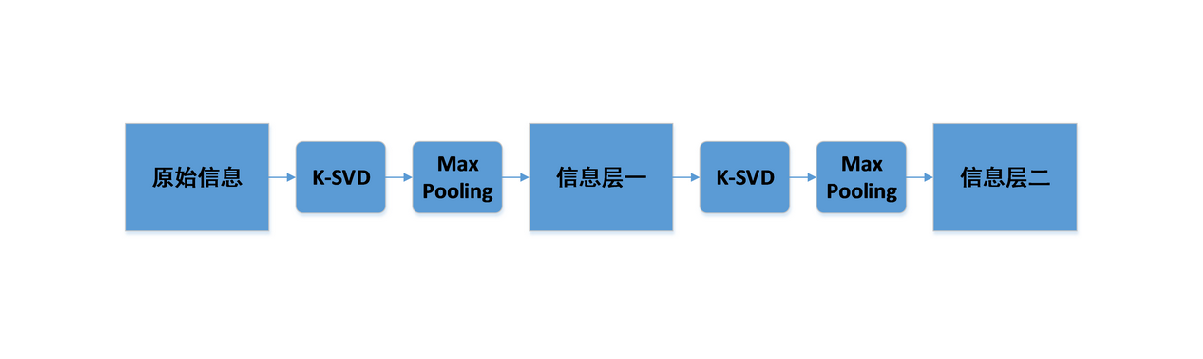
\includegraphics[width=1\textwidth]{workflow_HMP}
  \caption{分层匹配追踪的工作流}
  \label{fig:workflow_HMP}
\end{figure}

分层匹配追踪(HMP)~\inlinecite{bo2011hierarchical} 的中心概念是自动地学习低层和中层的特征,而不是使用人工选择的特征,例如SIFT~\inlinecite{ng2003sift} 等。HMP从原始数据中学习到一组稀疏字典,并使用这些字典给数据分层地编码,获得一个空间金字塔。如图~\ref{fig:workflow_HMP} 所示。具体地说,给定一组h维的观测值$Y = [y_1, ..., y_n] \in R^{h\times n}$,K-SVD的学习目标是找到一组字典$D = [d_1, ..., d_m] \in R^{m \times n}$(这里的$d_i$可以称为过滤器),和一组稀疏编码$X = [x_1, ..., x_n] \in R^{m \times n}$,使得如下重建误差最小化:
\begin{equation}
\label{equ:ksvd_minimize}
\underset{D,X}{\min}{||Y-DX||_F^2} \qquad s.t. ~ \forall i,~ ||x_i||_0 \leq K
\end{equation}
其中$||X||_F$表示X的弗罗贝尼乌斯范数(Frobenius norm);$x_i$是$X$的一列;$||*||_0$是零范数,数值等于$x_i$中为零项的个数;$K$是稀疏级别,表示每一组数据中为零项个数的上限。因为~\ref{equ:ksvd_minimize} 中的问题是非凸的,很难给出精确解,所以在实际操作中我们采用近似解法OMP~\inlinecite{aharon2006img} 来贪心地求解。具体地说,OMP会迭代地交替执行以下两个过程,逐步逼近最终结果。
$$
\underset{X}{\min}{||Y-D^*X||_F^2}
$$
$$
\underset{X}{\min}{||Y-DX^*||_F^2}
$$

通过K-SVD的提取出来的信息,可以较好地重构出原来的图片,如图\ref{fig:ksvd_rebuild}所示。重构出的图片与原图质量相差无几,说明尽管在使用分层匹配追踪时信息的维度和结构发生了较大变化,但大部分有用信息都被保留了下来。

\begin{figure}[H] % use float package if you want it here
  \centering
  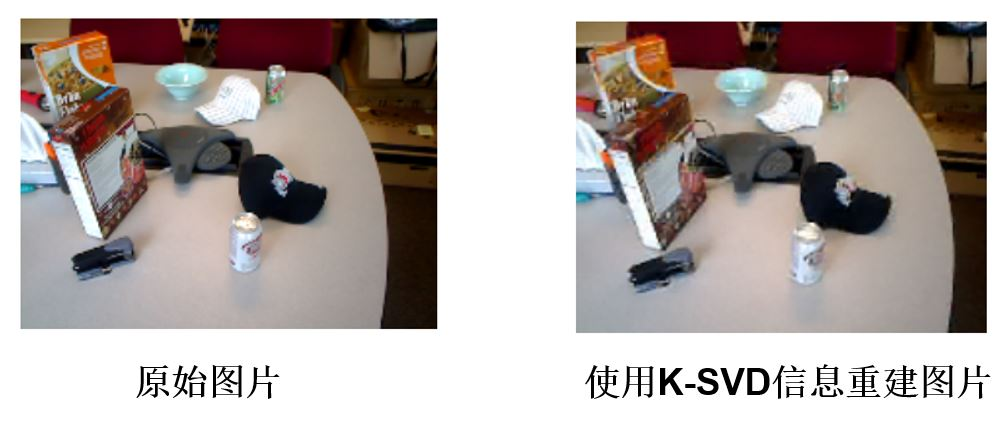
\includegraphics[width=0.9\textwidth]{ksvd_rebuild}
  \caption{K-SVD 保留信息可视化}
  \label{fig:ksvd_rebuild}
\end{figure}

如果将K-SVD学习得到的字典可视化,可以得到如图\ref{fig:ksvd_dict}所示的效果,可以看出:在深度、颜色信息之中学习到的字典(过滤器)均包含一定的有规律可循的模式,比如说边、角、点。其中RGB图片的字典含有颜色信息,而深度图片学习到的字典虽然没有颜色信息,但是边角分界处往往更加锋利清晰,这也体现了两种模态信息的互补性。

空间金字塔最大池化(Spatial pyramid max pooling)是一种高度非线性的信息处理过程,可以从局部稀疏编码中生成更高层次、更低维度的表征方式。它的结构如图~\ref{fig:maxpooling}所示~\inlinecite{yang2009linear}。
这种方法在多个层次上递归地进行最大池化。具体地说,假设最大池化的接受域为$2 \times 2$,那么第零层每个单元就代表原始数据中的一个单元,第一层每个单元代表原始数据中的四个单元,以此类推。设$U$为池化前的数据,$U$的每一列为原始数据中的邻域,$z$代表着池化之后的数据,那么最大池化可以表示为:

\begin{equation}
\begin{aligned}
z &= F(U) \\
z_j &= max\left\{|u_{1j}|, ..., |u_{Mj}|\right\}
\end{aligned}
\end{equation}

\begin{figure}[H] % use float package if you want it here
  \centering
  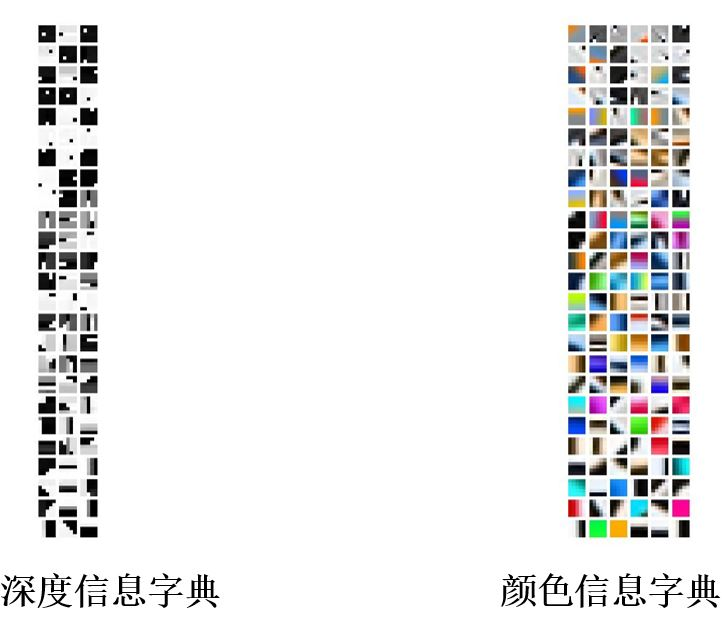
\includegraphics[width=0.65\textwidth]{ksvd_dict}
  \caption{K-SVD 字典可视化}
  \label{fig:ksvd_dict}
\end{figure}

\begin{figure}[H] % use float package if you want it here
  \centering
  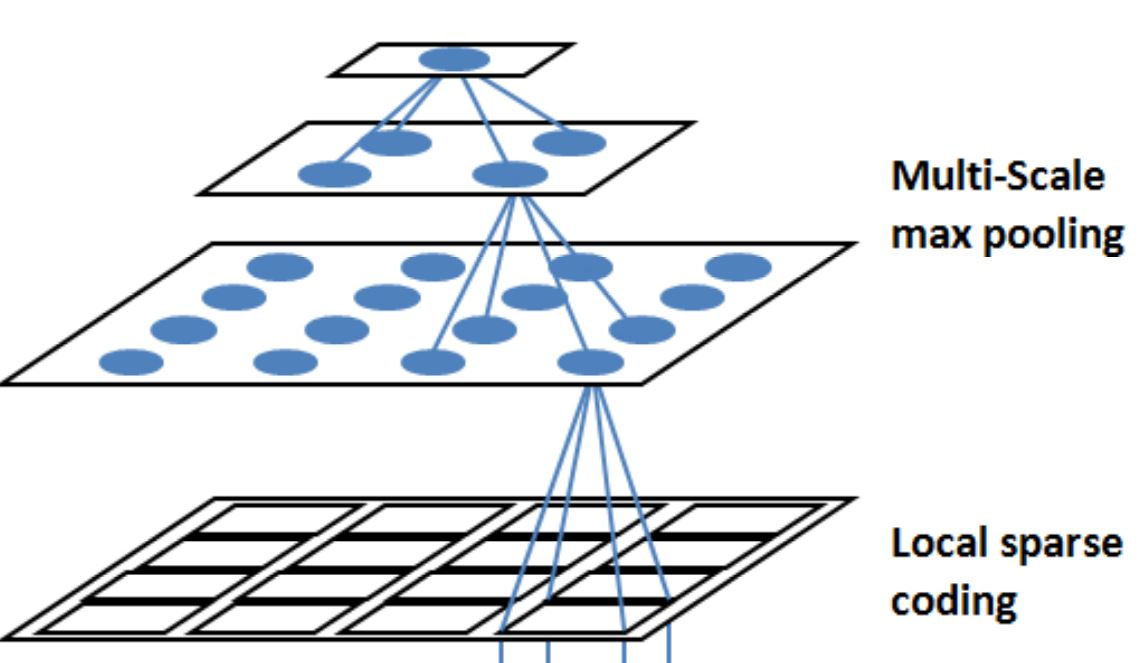
\includegraphics[width=0.8\textwidth]{maxpooling}
  \caption{空间金字塔最大池化示意图}
  \label{fig:maxpooling}
\end{figure}

具体的参数及实验效果见~\ref{sec:fStrategyExp} 小节。



\section{随机权值神经网络}
\label{sec:CRNN}

如果说分层匹配追踪是一种目的明确的监督学习(supervised learning),那么随机权值神经网络(CRNN)的信息提取过程就显得比较“随意”。在这里,我们引入CRNN作为另一种参与融合的信息提取策略,一方面是因为它可以引入一定的随机性,另一方面是因为通过神经网络的信息提取过程与传统的词袋模型(Bag of Words)具有很大不同,提取出的信息在结构上也与之有较大差别,所以可以预见CRNN与传统信息提取方法有着较大的互补性,将它们融合可以获得较大的准确率上的提升。由于一定随机性在许多人工智能策略中都可以避免陷入局部最优,提升策略表现,比如遗传算法~\inlinecite{goldberg1988genetic} 和蒙特卡洛方法~\inlinecite{metropolis1949monte} 等。所以我们也试图使用CRNN来给我们的模型引入一定的随机性。CRNN的工作流程图如图\ref{fig:workflow_CRNN} 所示。


\begin{figure}[H] % use float package if you want it here
  \centering
  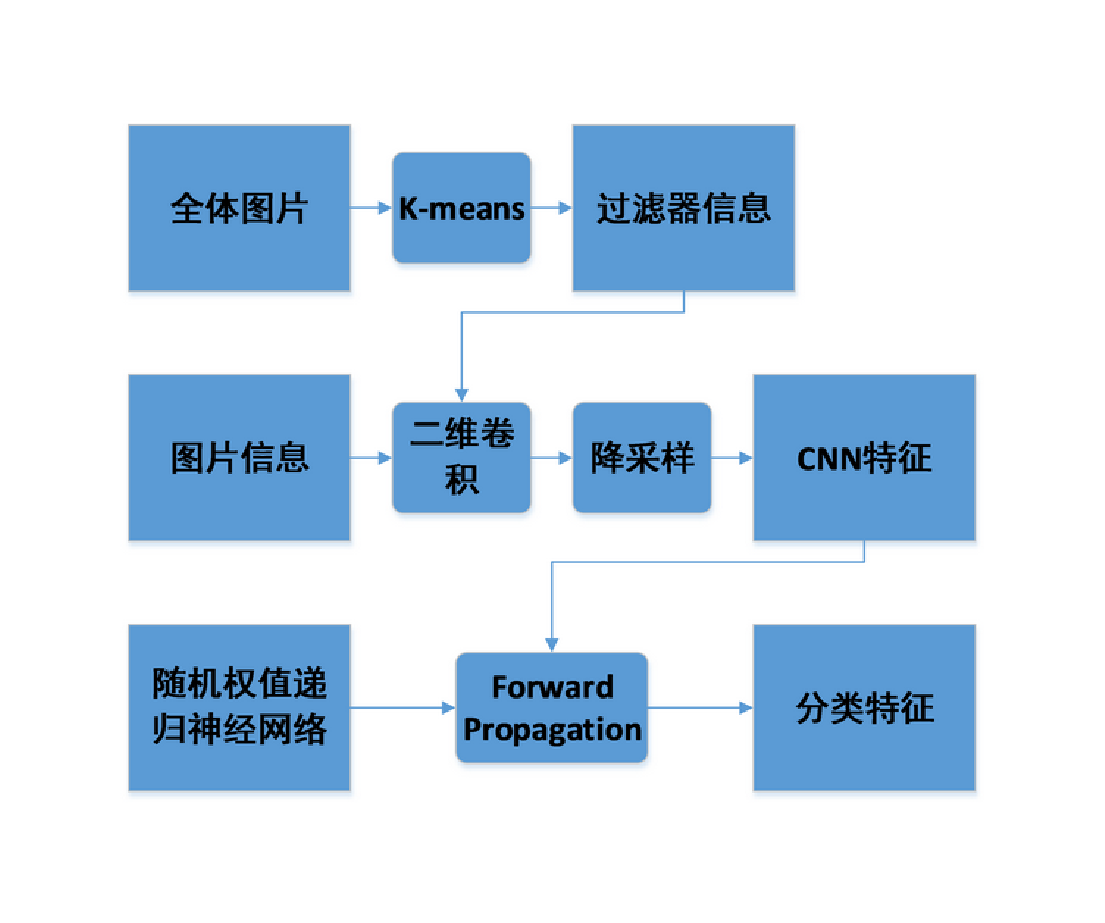
\includegraphics[width=0.95\textwidth]{workflow_CRNN}
  \caption{CRNN的的工作流}
  \label{fig:workflow_CRNN}
\end{figure}

如图\ref{fig:workflow_CRNN}所示,我们需要先得到一组过滤器,这个过滤器不一定需要在我们的训练集上学习出来,也可以在更大、更全面的数据集上预先通过K-means学习出来。
K-means的目标函数是:
\begin{equation}
\underset{S}{\min}\sum\limits_{i=1}^{k}{\sum\limits_{x \in S_i}{||x-\mu_i||^2}}
\end{equation}
其中k是K-means产生的中心的数量,S是分类信息,$\mu_i$是K-means产生的中心,$x \in S_i$说明信息x以$\mu_i$为中心。学习到的过滤器如图~\ref{fig:CNN_filters}所示。

\begin{figure}[H] % use float package if you want it here
  \centering
  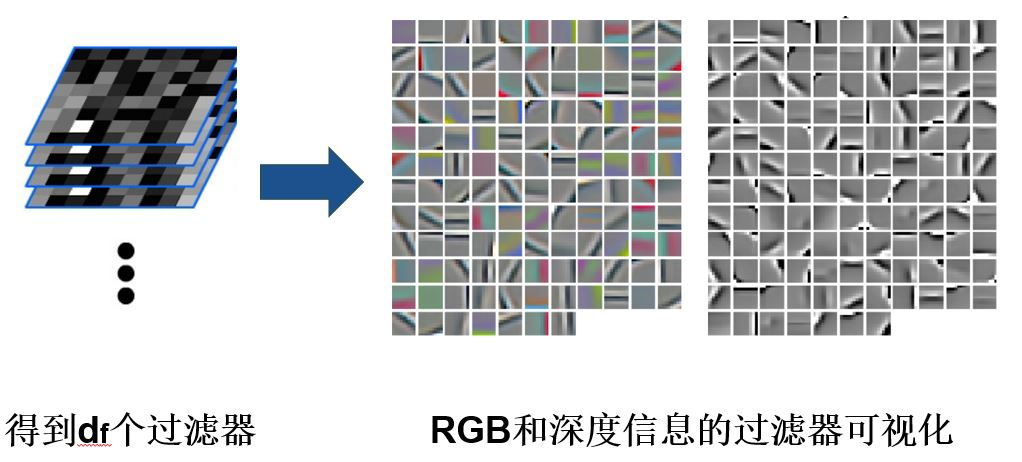
\includegraphics[width=0.95\textwidth]{CNN_filters}
  \caption{CNN的过滤器可视化}
  \label{fig:CNN_filters}
\end{figure}

然后我们使用Pretrained的过滤器信息与图片信息进行二维卷积和降采样,如图~\ref{fig:CNN_structure} 所示,以便得到图片的CNN特征。

由于我们使用一组过滤器分别与原图片卷积,所以对于每一张图片输入会得到一组CNN的模式(pattern)。通过CNN提取出的某个目标物体(一个苹果)的pattern如图~\ref{fig:CNN_feature}所示。可以看出,左边的RGB pattern含有一定的光照、纹理信息;而右边的Depth pattern则含有更加锋利明显的边界信息,这也体现了两种模态信息的互补性。

\begin{figure}[H] % use float package if you want it here
  \centering
  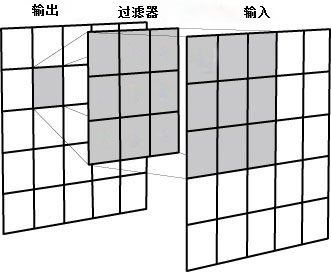
\includegraphics[width=0.8\textwidth]{CNN_structure}
  \caption{CNN的结构}
  \label{fig:CNN_structure}
\end{figure}

\begin{figure}[H] % use float package if you want it here
  \centering
  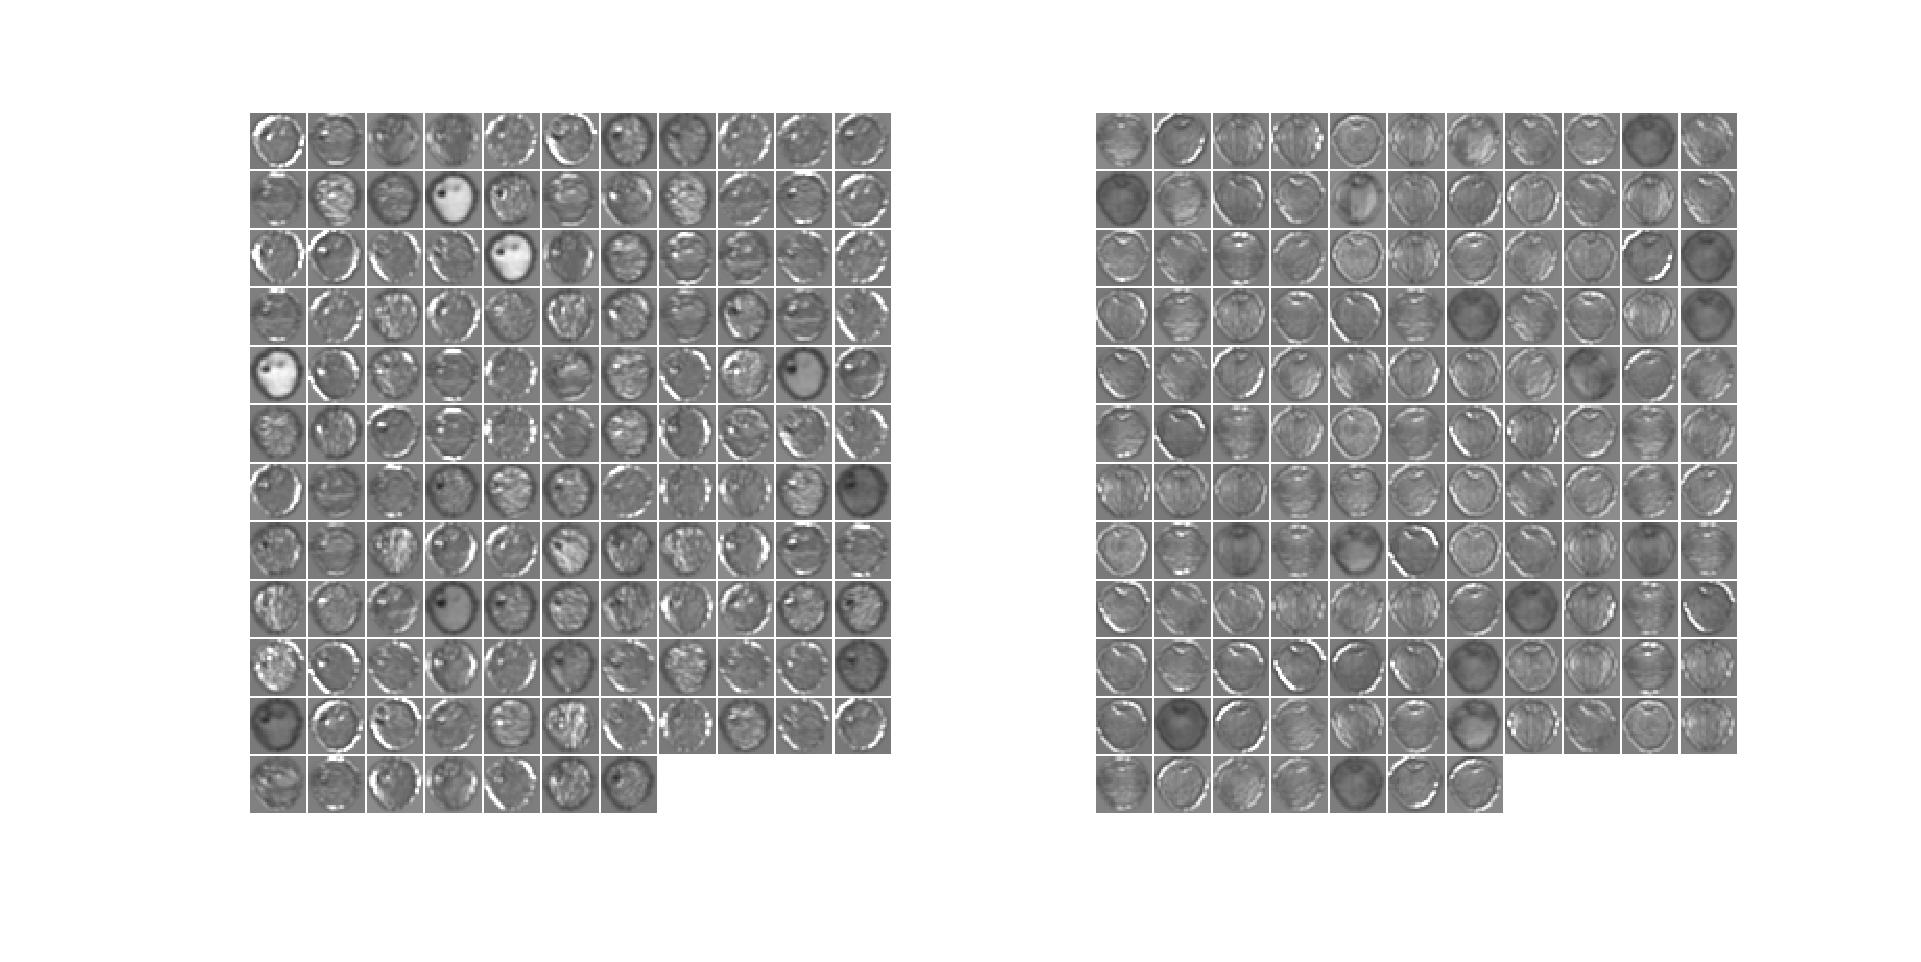
\includegraphics[width=1.1\textwidth]{CNN_feature}
  \caption{CNN所提取出的模式(左为RGB patter,右为Depth patter)}
  \label{fig:CNN_feature}
\end{figure}

然后我们将得到的CNN模式输入一组递归神经网络(RNN)。注意,这里我们虽然使用了神经网络,但是由于其权值是随机产生的,不会在信息提取的过程中改变,并且我们只使用前向传递(forward propagation)而不使用后向传递(back propagation),所以这并不是一个监督学习的过程,而是一个非监督(unsupervised)的信息提取过程。在这一步中我们对于每一层的每个接受域(相近的指定大小的区域)中的数值施加一个变换,得到一个数值作为更高层相应单元中的数值。具体地说:
\begin{equation}
\label{equ:RNN}
x_i^h = f(X_i^{h-1})
\end{equation}
其中,$x_i^h$代表h层的单元i的数值,$X_i^{h-1}$代表h层的单元i在h-1层对应的接受域内的数值矩阵。可以看出,RNN其实是空间金字塔最大池化(Spatial pyramid max pooling)的推广——将~\ref{equ:RNN} 式中的$f()$函数设置为取$max$就是空间金字塔最大池化。不过我们在分类时往往只使用上层的信息。RNN的工作示意图如图~\ref{fig:RNN_structure} 所示。


\begin{figure}[H] % use float package if you want it here
  \centering
  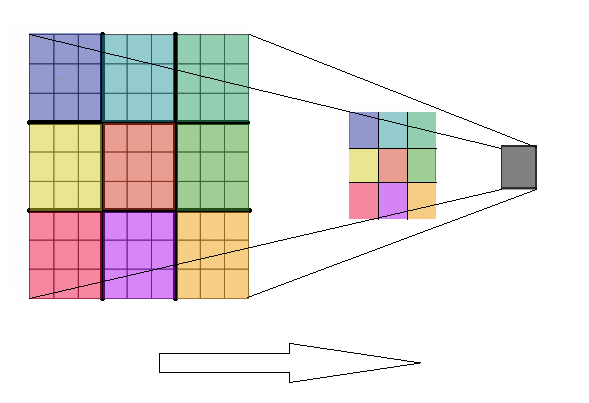
\includegraphics[width=0.95\textwidth]{RNN_structure}
  \caption{RNN工作示意图}
  \label{fig:RNN_structure}
\end{figure}

具体的参数及实验效果见~\ref{sec:fStrategyExp} 小节。


\section{多模态融合策略}
\label{sec:fStrategy}

\subsection{特征层融合}
\label{subsec:fInMethod}

对于同一方法内,不同模态间的信息融合,我们倾向于使用特征层的融合策略。因为正如前文所述,RGB信息和深度信息有着天然的互补性,而这些互补性在特征层体现得最明显。如果我们先分别利用颜色信息和深度信息得到一个分类的估计值,这样虽然具有了一定的语义信息,也可以从贝叶斯的角度来增大最终分类的准确率,但是这样就不能完全挖掘颜色和深度信息之间的联系与互补性。在实验中我们尝试了使用决策层的融合策略和特征层的融合策略,发现对于同一方法内的融合,在特征层的操作确实在大多数情况下会取得更好的结果。

具体地说,我们使用连接作为特征层融合的方法:
\begin{equation}
\label{equ:feature_level}
X_{feature} = [X_{RGB}, X_{D}]
\end{equation}
其中$X_{feature}$是特征层融合得到的信息,$X_{RGB}$是颜色图片提取出的信息,$X_{D}$是深度图片提取出的信息。

\subsection{决策层融合}
\label{subsec:fBetweenMethod}

而对于不同方法之间的信息融合,我们更倾向于使用决策层的融合策略。原因如下:
\begin{enumerate}
\item 由于方法的不同,各组特征之间维度差异较大,在特征层难以权衡各个方法在总体决策中占的权重,维数越高的信息在特征层融合之后占总体决策权重就会越大。
\item 各组特征结构差异较大,如果使用特征层融合,难以捕捉其中的联系。相反,有可能造成过拟合。
\item 由于在特征层融合之后特征的维度往往比较高,对于接下来的决策步骤中的计算资源要求也较高。而采用决策层融合的策略可以分而治之,将特征压缩为带有语义的信息再做处理。
\end{enumerate}

在实验中,由于需要两个分类器带权投票,我们需要能够产生分类自信度的分类器,所以优先试验了贝叶斯分类器。但是发现贝叶斯分类器在信息矩阵维数较高时计算过于缓慢,且效果也不如SVM。所以我们决定使用SVM分类器来进行分类决策。不过因为原生的SVM只能够产生分类结果,而不能产生分类自信度,为了实现决策级的信息融合,我们使用Sigmoid-Softmax方法将SVM的决策值转化为自信度估计,如~\ref{equ:sigmoid_softmax} 式所示。

\begin{equation}
\label{equ:sigmoid_softmax}
P(C_j|I_i) = \frac{Sigmoid(dec\_value_{ij})}{\underset{k}{\sum}{Sigmoid(dec\_value_{ik})}}
\end{equation}

最终,我们在使用~\ref{equ:sigmoid_softmax} 式得出两种方法各自的分类自信度之后投票决定最终输出结果。实验证明,我们提出的融合策略可以有效地捕捉方法间的信息互补性,使得最终分类结果有所提升。整体融合策略的框架如图~\ref{fig:workflow_fstrategy} 所示。

\begin{figure}[H] % use float package if you want it here
  \centering
  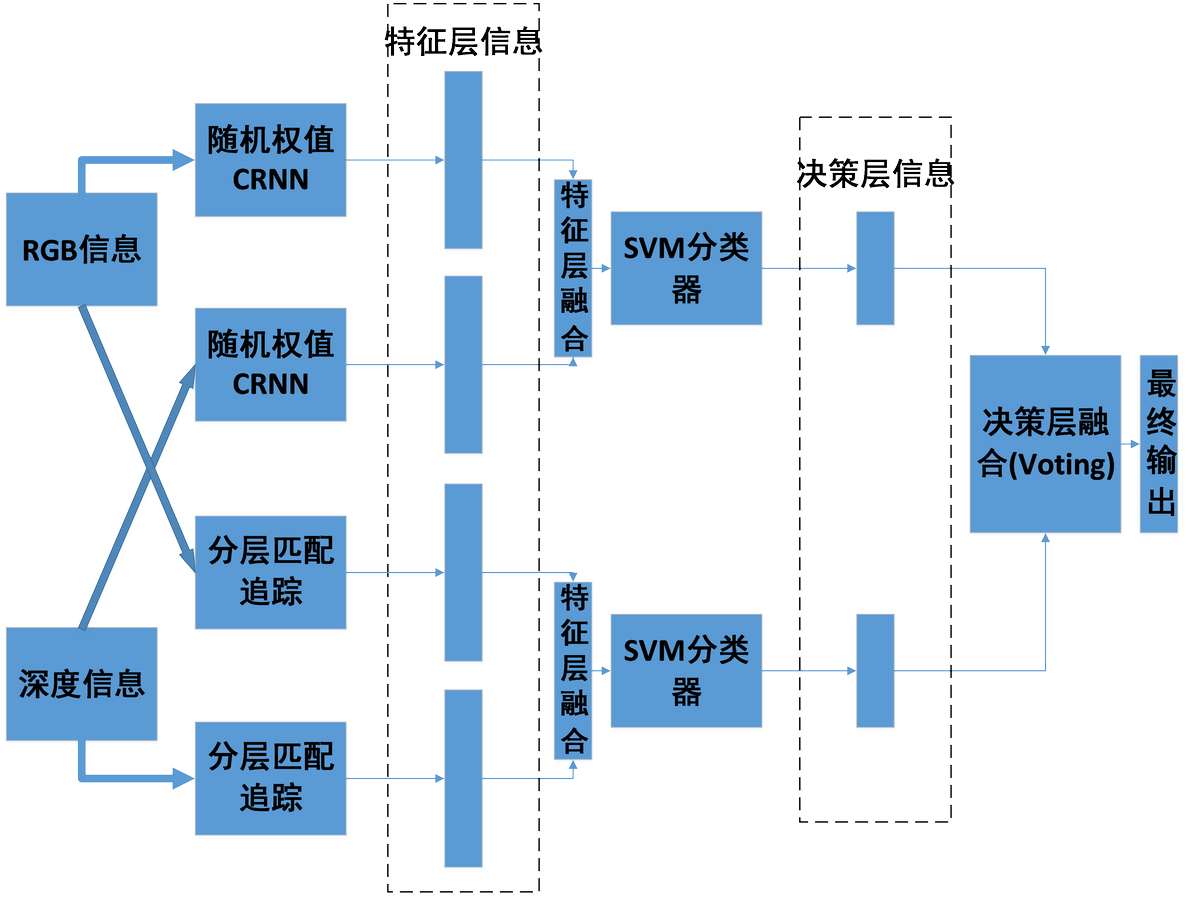
\includegraphics[width=0.95\textwidth]{workflow_fstrategy}
  \caption{整体融合策略的框架}
  \label{fig:workflow_fstrategy}
\end{figure}

具体的参数及实验效果见~\ref{sec:fStrategyExp} 小节。


\section{试验验证}
\label{sec:fStrategyExp}

\subsection{试验综述}

我们选用了上文中提到的华盛顿大学RGB-D数据集~\inlinecite{lai2011large} 作为我们的训练集。此数据集包含分别属于51个类别的日常用品的300个物体实例,如图~\ref{fig:washington}所示。总共包含超过20万组匹配的RGB-D图片,在实验中我们为了与~\inlinecite{lai2011large} 的baseline对比,所以选用了其中的41877组RGB-D信息。

\begin{figure}[H] % use float package if you want it here
  \centering
  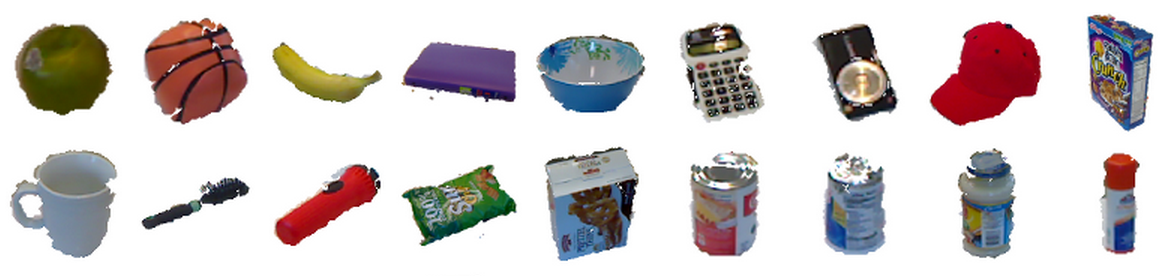
\includegraphics[width=0.95\textwidth]{washington}
  \caption{华盛顿RGB-D数据集}
  \label{fig:washington}
\end{figure}

在本节中我们对颜色信息和深度信息分别用CRNN和HMP两种方法进行分类,然后将两种模态在不同层次融合起来进行分类,以观察模态间融合的效果提升。然后我们为了探究不同模态之间的互补性,对比了两种模态的混淆矩阵,并对其中典型的例子进行了探讨。最后我们统一使用RGB-D信息,用两种方法进行分类并尝试在不同层次进行融合,以探究方法融合的效果。其中SVM分类器的实现我们选择使用 liblinear~\inlinecite{REF08a} 。

\subsection{试验参数}

对于分层匹配追踪,我们需要在两个层次上设置相应的参数。

第一层。从1000000个$5 \times 5$的深度图片样本中学习出75组稀疏度为5的灰度字典和深度字典;从1000000个$5 \times 5 \times 3$的RGB图片样本中学习出150组稀疏度为5的颜色字典和曲面法线字典。接下来我们使用上述字典,使用OMP算出原图对应的稀疏编码,并使用空间金字塔最大池化的方法产生$16 \times 16$,$4 \times 4$,$2 \times 2$,$1 \times 1$的信息,将它们拼接在一起压缩成一维,作为第一层的输出特征。

第二层。在第一层输出的基础上从1000000个$5 \times 5$的深度图片和RGB图片产生的输出特征中学习出1000组稀疏度为10的灰度字典、深度字典、颜色字典和曲面法线字典。接下来我们使用上述字典,使用OMP算出第一层输出对应的稀疏编码,并使用空间金字塔最大池化的方法产生$3 \times 3$,$2 \times 2$,$1 \times 1$的分割信息,将它们拼接在一起压缩成一维,得到总共$4(channel) \times 1000(dict) \times (3 \times 3 + 2 \times 2 + 1 \times 1) = 54000$维向量,作为第一层的输出特征(其中RGB和深度信息分别为28000维)。因为第一层信息维度过高,所以在实验中我们只使用第二层的信息。

对于CRNN,我们同样需要在两个层次上设置参数。

CNN层。学习出128个过滤器,分别和RGB和深度图片卷积之后降采样得到$27 \times 27$的图片块,所以对于每一张RGB或深度图片分别可以得到$128 \times 27 \times 27$的图片块(见图片~\ref{fig:CNN_feature})。

RNN层。利用CNN层得到的维度为$128 \times 27 \times 27$的图片块,将每一个过滤器对应的$27 \times 27$的图片块分别通过128个随机产生的RNN,每个RNN得到 $1 \times 1$ 维特征。所以最终我们得到每张RGB和深度图片对应的信息分别为$128 \times 128 = 16384$维,总共有32768维输出信息。

\subsection{试验结果}

在实验中,我们采用以上的参数设置,得到如下实验结果:

\begin{table}[htbp]
  \centering
  \caption{模态间融合实验结果}
  \label{tab:fStrategyResult1}
  \begin{minipage}[t]{0.8\textwidth} 
    \begin{tabularx}{\linewidth}{|l|X|X|X|X|}
      \hline
 \multirow{2}*{\diagbox[width=5em]{方法}{模态}} & \multirow{2}*{RGB} & \multirow{2}*{Depth} & \multicolumn{2}{c|}{RGB \& Depth}\\\cline{4-5}
      & & &特征融合$^{*}$&决策融合$^{**}$ \\ \hline
      CRNN      & $81.7 \pm 1.4$ & $78.9 \pm 1.6$ & $\boldsymbol{87.6 \pm 1.2}$ & $87.3 \pm 1.1$ \\
      HMP       & $75.8 \pm 3.4$ & $78.4 \pm 1.9$ & $85.4 \pm 2.6$ & $\boldsymbol{86.3 \pm 2.1}$ \\
      决策融合  & $83.1 \pm 2.6$ & $82.5 \pm 1.9$ & $\boldsymbol{89.6 \pm 2.1}$ & $89.1 \pm 1.8$ \\ \hline
    \end{tabularx}\\[2pt]
    \footnotesize
    *:使用~\ref{equ:feature_level} 式\\
    **:使用~\ref{equ:sigmoid_softmax} 式
  \end{minipage}
\end{table}

通过表~\ref{tab:fStrategyResult1} 我们可以看出,多模态信息融合可以明显提升分类准确率。下面我们以匹配追踪为例,来探究两种模态的信息互补性。两种模态信息分类的混淆矩阵(Confusion Matrix)如图~\ref{fig:confusion_matrix} 所示。混淆矩阵~\inlinecite{townsend1971theoretical} 是在监督学习中对于分类结果的可视化,其每一列表示了一个预测类别;其每一行表示了一个真实类别,一个数据实例属于第i行第j列当且仅当此实例数据第i类,被分类模型分到第j类。颜色越深的区域中含分类实例越多,所以理想化的混淆矩阵应该是对角矩阵。通过对两者混淆矩阵的比较可以看出,它们是有一定的互补性的。例如图片~\ref{fig:instance} 所示,如果只使用深度信息,容易将peach分类为sponge,如果只使用颜色信息,又容易将sponge分类为rubber eraser。而将两种信息结合起来之后,上述三种物品均可以得到较好分类。

\begin{figure}[H] % use float package if you want it here
  \centering
  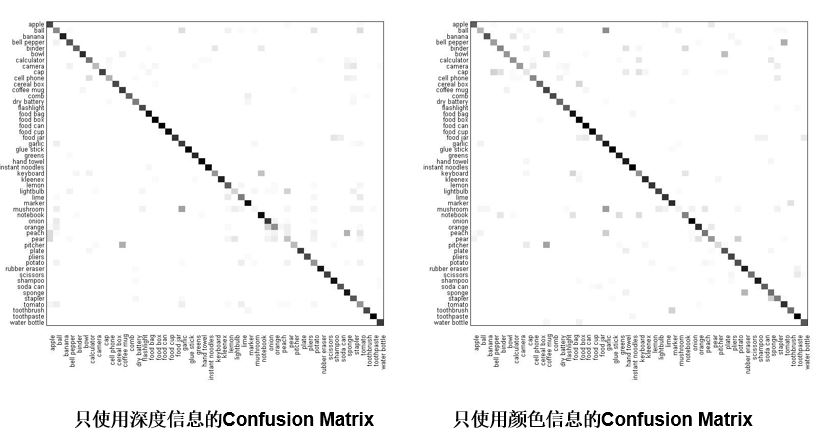
\includegraphics[width=0.95\textwidth]{confusion_matrix}
  \caption{两种模态信息分类的混淆矩阵}
  \label{fig:confusion_matrix}
\end{figure}

\begin{figure}[H] % use float package if you want it here
  \centering
  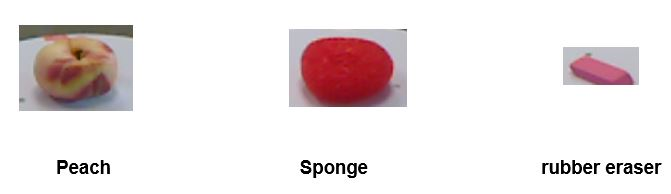
\includegraphics[width=0.95\textwidth]{instance}
  \caption{分类效果举例}
  \label{fig:instance}
\end{figure}

\begin{table}[htbp]
  \centering
  \caption{方法间融合实验结果}
  \label{tab:fStrategyResult2}
  \begin{minipage}[t]{0.8\textwidth} 
    \begin{tabularx}{\linewidth}{|X|X|X|X|}
      \hline
      CRNN & HMP & CRNN \& HMP 特征融合$^{*}$ & CRNN \& HMP 决策融合$^{**}$ \\ \hline
      $87.6 \pm 1.2$ & $85.4 \pm 2.6$ & $88.7 \pm 2.0$ & $\boldsymbol{89.6 \pm 2.1}$ \\ \hline
    \end{tabularx}\\[2pt]
    \footnotesize
    本表展示的均是使用RGB-D信息得到的结果。\\
    *:使用~\ref{equ:feature_level} 式\\
    **:使用~\ref{equ:sigmoid_softmax} 式
  \end{minipage}
\end{table}

接下来我们使用RGB-D信息,探究两种信息提取方法之间的融合策略。得到结果如表~\ref{tab:fStrategyResult2} 所示。
可以看出,不论是模态间还是方法间的信息融合都可以明显提高分类的准确率。而且正如我们预测的一样,在方法间采用决策层的融合可以更好的提升效果。我们在图~\ref{fig:workflow_fstrategy} 中提出的融合模型,可以综合使用图~\ref{fig:workflow_HMP} 和图~\ref{fig:workflow_CRNN} 中的方法,并得到有效的效果提升。
\chapter{深度学习在多模态融合中的应用}
\label{cha:deeplearning}

本章主要介绍使用深度学习进行多模态信息融合的思路、具体操作和实验结果。随着深度学习的飞速发展,包括分类、识别、检测乃至决策判断等诸多任务的记录都已经被刷新。在图片的识别中深度学习更是大显身手,展示出了惊人的威力,早已超过了传统的机器学习做法。所以本文为了突破传统的 Bag of Words 信息提取与处理的局限,引入了深度学习方法。并且我们不是使用深度学习方法直接给出分类结果,而是使用深度学习的模型来提取特征层信息,然后使用SVM分类器进行分类。这样做的原因是为了便于和其他方法在多个层次上进行融合,更加具有拓展性。

此外,本文还提出了一种将深度信息转换为图片信息的深度信息自适应正规化(Depth adaptive normalization)。深度信息自适应正规化的核心思想是对于深度图片的不同组成部分(例如目标物体、背景、噪声等部分)采用不同的正规化尺度。这种方法的优势有:可以保留目标物体与次要部分(比如背景和噪声)之间的间隔,使得目标物体形状轮廓清晰可辨;同时可以保留甚至放大目标物体内部三维形状变化的信息,使得目标物体含有的信息更加具体丰满;还可以一定程度上降低噪声和背景等对于识别结果的干扰。这种方法相比于其他深度信息到图片的编码方法相比,计算量小,不需要任何额外的信息。且可以与其他编码方法结合使用,即在这种正规化的方法之上再加入其他的编码信息。

最后,因为深度学习对于数据量需求巨大,而我们使用的多模态匹配的数据集往往具有数据量不足,过拟合的现象。为了解决前述问题,我们使用了预先在当前最大的RGB图片数据集ImageNet~\inlinecite{deng2009imagenet} 中训练的模型来辅助信息提取。同时,由于已有模型的训练集只包含RGB图片,对于颜色信息我们可以直接使用原 Pretrained 模型,而对于深度信息的提取,我们尝试预先使用现有的深度图片信息对原有模型进行微调(finetune),使它更好地适应于深度信息的提取。


\section{深度学习模型描述}
\label{sec:dModel}

在实验中我们使用了八层的深度卷积神经网络 AlexNet~\inlinecite{krizhevsky2012imagenet} 在颜色信息和深度信息中分别进行深度学习训练出一个适用于RGB的模型和一个适用于深度信息的模型,然后使用相应的模型将高层特征提取出来,使用SVM分类器和~\ref{equ:sigmoid_softmax} 式做出决策并给出分类自信度。最后与其它分类模态在决策层进行融合。
引入深度学习的意义在于,Deep Learning 在许多方面可以与传统词袋信息提取方法互相补充,有助于突破传统方法的局限。同时,深度学习最终提取出的特征由于高度压缩,维度较小。最后,在数据规模足够大的时候,深度学习能够获得远高于词袋方法的分类及识别准确率。使用深度学习与传统方法互相补充,就好比使用一个新型的、更高精度的传感器与传统的传感器联合做出决策。

AlexNet 的结构如图~\ref{fig:AlexNet} 所示(图片引自~\inlinecite{krizhevsky2012imagenet})。在实验中,我们提取 AlexNet 决策层之前的两层(分别称为fc6和fc7)作为分类信息,将其提取出来并与其它特征进行融合。之所以选择这两层作为分类信息是因为以下原因:
\begin{enumerate}
\item 原模型第八层(最后一层)为决策层,会给出图片在1000个类别中的分类结果,且包含维度过少,有较大的信息损失。
\item 原模型第六层、第七层之前的信息层维数过高(例如:第五层含有 $13 \times 13 \times 128 \times 2 = 43264$ 维,数据冗余严重。而第六层第七层加起来一共只有 $2048 \times 4 = 8192$ 维)
\item 由于决策层实际上是一个SoftMax分类器,所以决策层之前的特征层的信息往往具有很好的可分性。
\end{enumerate}


\begin{figure}[H] % use float package if you want it here
  \centering
  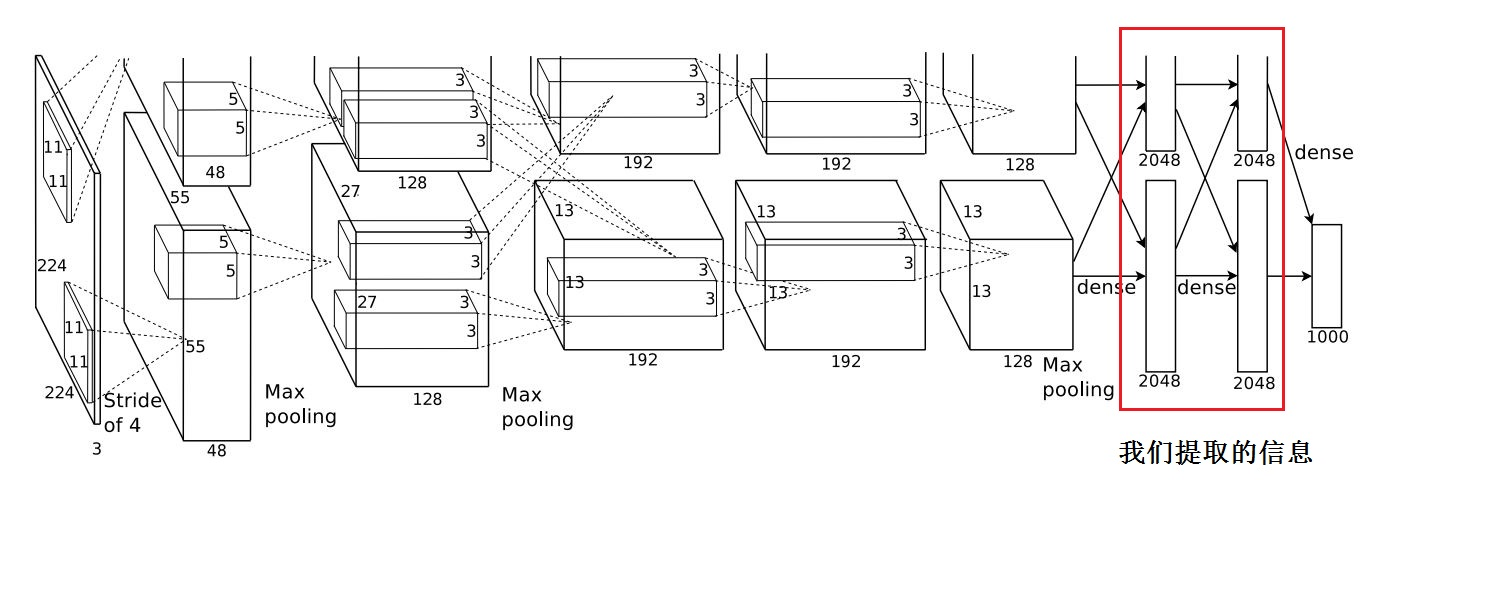
\includegraphics[width=0.95\textwidth]{AlexNet}
  \caption{AlexNet 结构示意图}
  \label{fig:AlexNet}
\end{figure}

使用上述步骤我已经可以成功地提取信息并得出分类结果。具体的参数及实验效果见~\ref{sec:deeplearningExp} 小节。


\section{Pretrained模型引入}
\label{sec:Pretrained}

在上一小节我们已经可以提取信息,不过分类效果并不是很好。这主要是因为如前所述,我们的深度学习模型因为数据量不足而发生了过拟合。所以,为了解决深度学习中数据量规模不足的问题,我们引入Pretrained模型作为辅助。我们使用的 AlexNet 模型,是 ILSVRC12 比赛中在 ImageNet 中训练出来的~\inlinecite{ILSVRC15}。

由于已有模型是在RGB图片数据集中训练的,我们在使用它处理深度信息之前一方面需要把深度信息转为合法的深度图片,另一方面会先使用已有Depth信息对其进行微调(Finetune),使它更好地适应Depth信息的提取工作。试验证明,使用RGB图片预先训练的深度学习模型可以较好地提取颜色和深度信息。使用已有模型进行微调比从头开始训练有如下好处:

\begin{enumerate}
\item 微调是在之前训练的结果的基础上继续训练,相当于数据集被扩大了,训练出的模型的表现也可以超过从头训练的模型。
\item 训练过程缩短,节省时间和资源。
\end{enumerate}

在微调过程中,我们保留 AlexNet 前七层的结构(如图~\ref{fig:AlexNet} 所示) 与参数,将第八层替换为一个输出维度为51的决策层(因为我们的数据共有51类)。以深度信息为例,从头训练与微调的训练损失(Training loss)和测试准确率(Test Accuracy)的变化对比如图~\ref{fig:training_loss} 和图~\ref{fig:accuracy} 所示,可见在微调中,原模型的训练损失迅速下降,测试准确率迅速上升,这说明原模型可以很快地适应新的数据集。

\begin{figure}[H] % use float package if you want it here
  \centering
  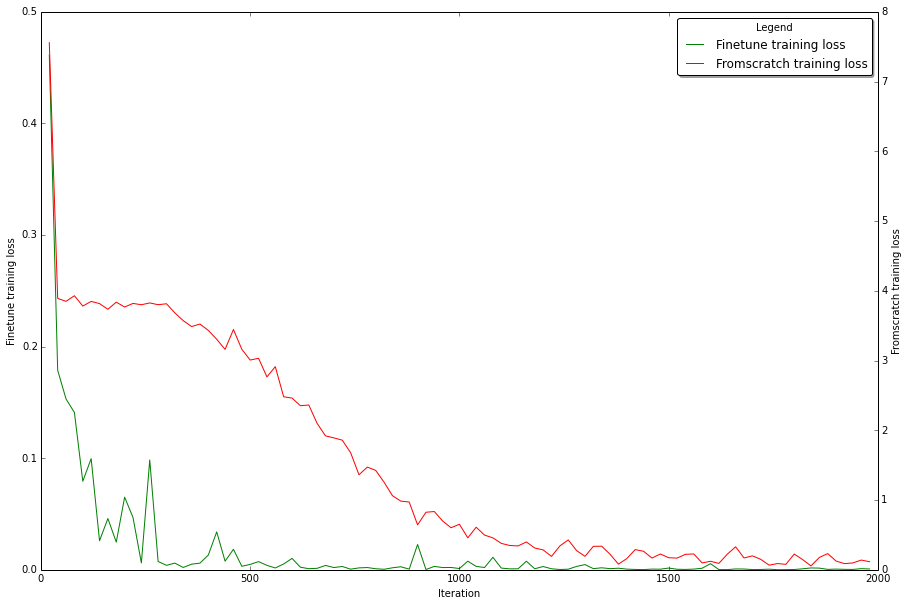
\includegraphics[width=0.95\textwidth]{training_loss}
  \caption{从头训练与微调的训练损失(Training loss)对比}
  \label{fig:training_loss}
\end{figure}

\begin{figure}[H] % use float package if you want it here
  \centering
  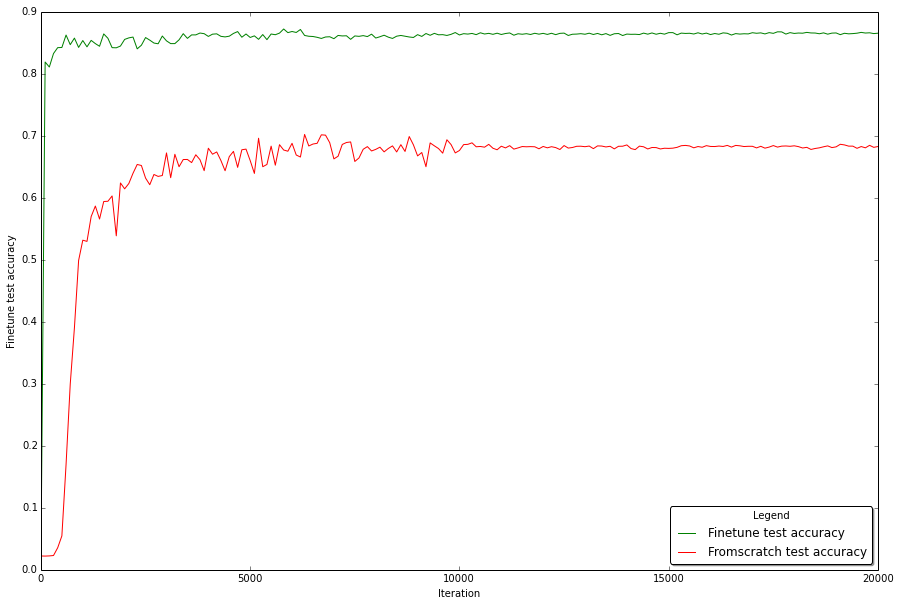
\includegraphics[width=0.95\textwidth]{accuracy}
  \caption{从头训练与微调的测试准确率(Test Accuracy)对比}
  \label{fig:accuracy}
\end{figure}

通过引入Pretrained模型,我们可以比较成功地提取RGB信息并获得85\%以上的准确率,已经接近HMP或CRNN方法中综合使用两种模态信息的表现。具体的参数及实验效果见~\ref{sec:deeplearningExp} 小节。

\section{深度信息自适应正规化}
\label{sec:dNorm}

通过引入Pretrained模型,我们已经成功地提取出RGB信息并只使用RGB信息获得85\%以上的识别准确率。然而使用深度信息效果却不甚理想,经过研究发现,这是因为我直接将深度图片传入了 Caffe 而没有将它们正规化为合法的图片。
由于深度信息是由单通道的深度数值构成的,而且每一个像素点上的数值范围可能不合法。而合法图片信息是由三通道构成的,且每一个像素点的数值在$[0-255]$之间。所以我就把深度图片正规化到了$[0-255]$之间,并将单通道扩展为三通道。不过这样做之后效果仍然不好。所以我又尝试了一些的预处理方法,比如说试图使用一些mask把背景遮住,或者使用interpolation把深度信息中的噪声点都修补上,但是效果都善乏可陈。

最后我想到,可能是正常的正规化的过程使得深度的“纹理”信息有损失。例如,原始深度图片上,物体的深度分布在$[720-780]$之间,而背景的深度分布在$[2000-3000]$之间,噪声的深度接近0。而如果把这张深度图normalize到$[0-255]$之间的话,原来分布在$[720-780]$之间的物体信息就变成了$[\frac{720}{3000} \times 255 - \frac{780}{3000} \times 255] = [61.2, 66.3]$之间,也就是说物体自身上的深度差异很大程度上被忽略了;当然,这样做也有好处,就是物体和背景之间的gap特别大,但是我觉得适当缩小gap并不会影响物体形状轮廓的可辨识度。

所以我提出了一种{\heiti 深度信息自适应正规化方法} (Depth Adaptive Normalization, DAN),会有选择地保留、加重、淡化、忽略某些信息。规范化的描述见算法~\ref{alg:DAN}。

\begin{algorithm}
  \caption{Depth Adaptive Normalization}
  \label{alg:DAN}
  \begin{algorithmic}[1]
    \REQUIRE DepthMap $\in R^{n \times m}$,\quad MaxGapNear,\quad MaxGapFar,\quad ThresholdGap
    \STATE $DepthArray \gets Squeeze(DepthMap)$
    \STATE $DepthArray \gets Sort(Unique(DepthArray))$
    \STATE targetNear $\gets$ min(DepthArray),\quad targetFar $\gets$ max(DepthArray)
    % Find the two gaps
    \\ \textbf{Find the two gaps}
    \FOR {$e_i$ in DepthArray}
      \IF {$e_i$ - $e_{i-1}$ > ThresholdGap}
        \IF {targetNear == -1}
          \STATE {targetNear $\gets e_{i}$}
        \ELSE
          \STATE {targetFar $\gets e_{i-1}$}
        \ENDIF
      \ENDIF
    \ENDFOR
    % Normalize the two gaps
    \\ \textbf{Normalize the two gaps}
    \FOR {$e_i$ in DepthMap}
      \IF {$e_i$ < targetNear}
        \STATE {$e_i \gets$ 0}
      \ELSIF {$e_i$ > targetFar}
        \STATE {$e_i \gets$ (targetFar - targetNear) + MaxGapNear + MaxGapFar}
      \ELSE
        \STATE {$e_i \gets e_i$ - (targetNear + MaxGapNear)}
      \ENDIF
    \ENDFOR
  \end{algorithmic}
\end{algorithm}

具体地说,就是先根据明显的Gap将深度信息划分为几个部分,然后根据需要保留相应的部分(比如目标物体信息),忽略不需要的部分(比如gap,背景信息),如图~\ref{fig:DAN} 所示。

\begin{figure}[H] % use float package if you want it here
  \centering
  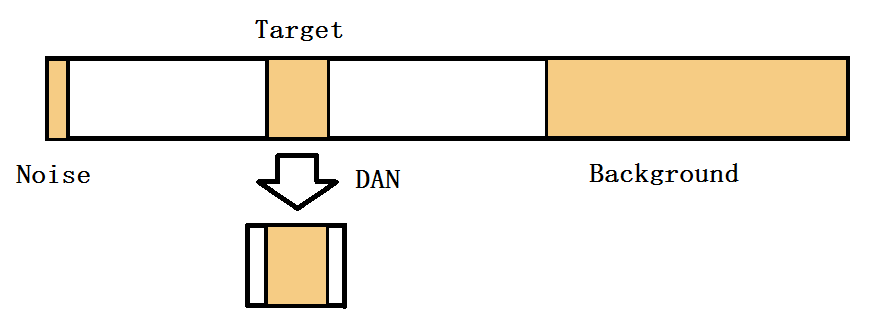
\includegraphics[width=0.95\textwidth]{DAN}
  \caption{深度信息自适应正规化方法示意图}
  \label{fig:DAN}
\end{figure}

比如说上例中,设置 $MaxGap = 20$。 0到720之间gap为720,把它缩小到20,780到2000之间gap为1280,把它缩小到20,2000到3000之间很容易判断为背景,所以这部分数值都用2000代替(不需要考虑背景的纹理)。所以最终深度信息变为$[0-20][20-80][80-100]$(其中[20-80]是原来的 $[720-780]$ 之间的物体信息),把这些信息再缩放到 $[0-255]$ 之间即完成了正规化。这样做的好处有:

\begin{enumerate}
\item 保留了目标物体与其他部分(比如背景和噪声)之间的间隔,使得目标物体形状轮廓清晰可辨。
\item 保留了(有时甚至可能放大)目标物体内部三维形状变化的信息,使得目标物体含有的信息更加具体丰满。
\item 一定程度上忽略了噪声、背景对于识别效果的干扰。
\end{enumerate}

具体的,我们将算法~\ref{alg:DAN} 中的 MaxGapNear 和 MaxGapFar 设为 5,ThresholdGap 设为100,在对水壶的深度信息处理之后可以可到的的深度图像如图~\ref{fig:DANresult} 所示,而不使用DAN得到的深度图像如图~\ref{fig:noDANresult} 所示。图~\ref{fig:DANresult} 包含了更加细致的水壶壶身弧度的变化,所以显然包含更加详细的深度信息。

\begin{figure}[htbp]
\begin{minipage}{0.48\textwidth}
  \centering
  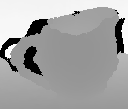
\includegraphics{pitchernonorm}
  \caption{使用普通正规化得到的深度图像}
  \label{fig:noDANresult}
\end{minipage}\hfill
\begin{minipage}{0.48\textwidth}
  \centering
  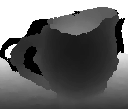
\includegraphics{pitcher20}
  \caption{使用DAN得到的深度图像}
  \label{fig:DANresult}
\end{minipage}
\caption{深度信息自适应正规化效果}
\label{fig:DANcompare}
\end{figure}

通过本小节介绍的深度信息自适应正规化方法,我们可以成功提取深度信息并获得80\%以上的分类准确率。具体的参数及实验效果见~\ref{sec:deeplearningExp} 小节。

\section{试验验证}
\label{sec:deeplearningExp}

\subsection{试验综述}

华盛顿大学RGB-D数据集的物体由41877个含家用物品的RGB-D图像组织成,它们分别属于51个不同的种类和一共300个实例,这些图像是在三个不同视点捕捉的。我们使用间隔5帧的采样来评估我们的算法。我们使用和Lai等
人~\inlinecite{lai2011large} 相同的十折交叉验证分割,来评估我们的方法在类别识别任务中的表现。每个分割包括大约35000组训练RGB-D数据和7000组测试RGB-D数据。在每个分割中,每一个对象类中都有一个实例是被留下做测试的。所以我们在剩下的 300-51 = 249 个实例中进行训练。在测试时任务是给每个之前没见过的实例分类。

我们使用了开源的深度学习框架——Caffe~\inlinecite{jia2014caffe} 来完成我们深度学习的试验。
同时,我们使用Krizhevsky等人~\inlinecite{krizhevsky2012imagenet}训练的AlexNet作为预训练模型。
为了使得结果更加清晰,本章的试验采用控制变量法的方式展现。分别根据:深度学习方法(是否使用预训练的模型、是否使用深度信息自适应正规化),使用的AlexNet中的信息层(第六层、第七层、两层结合),以及微调(是否微调)为变量展示了相关实验结果。特征层融合使用的是~\ref{subsec:fInMethod} 小节中介绍的方法,决策层融合使用的是~\ref{subsec:fBetweenMethod} 小节中介绍的方法。


\subsection{试验参数}

如先前所描述,我们使用 AlexNet 作为我们融合网络的基础。它由五个卷积层(在第一、第二和第五之后需要最大池化),其次是两个完全连接层和SOFTMAX分类层。除了最后一层之外所有的层都用到了线性修正单元。
在从头训练的情境中,我们将所有信息层的参数都设置成按照一种固定学习率(learning rate)的模式在改变(最开始学习率取为0.01,经过40K次迭代后变为0.001,并在60K次迭代后停止训练)。

在微调过程中我们使用预先训练的模型的前七层(如图~\ref{fig:AlexNet} 所示)的权重和偏差来初始化我们网络的前七层,丢掉了最后的SOFTMAX分类层,将第八层替换为一个输出维度为51的决策层(因为我们的数据共有51类)。然后我们继续使用分阶段训练。在微调的情境中,我们将模型前七层的参数设置为按照一种固定学习率(learning rate)的模式在改变(最开始学习率取为0.001,经过10K次迭代后变为0.0001,并在20K次迭代后停止训练),将最后一层的学习率设置为始终是前七层的十倍(即最开始学习率取为0.01,经过10K次迭代后变为0.001,并在20K次迭代后停止训练)。这样设置的原因是前七层由于继承了原模型的参数,已经趋于稳定,需要改变的幅度较小;而第八层由于是从头训练,需要改变的幅度较大。我们尝试了微调RGB和深度信息,但是最后发现微调RGB信息并不能带来识别效果的改进。

未经特殊说明,我们将算法~\ref{alg:DAN} 中的 MaxGapNear 和 MaxGapFar 设为 5,ThresholdGap 设为100。

我们从此任务的十种数据分割方法中随机选出一种分割方法作为确认分割,而训练的迭代次数以及其他参数都是基于在确认分割上的测试结果所选定的。如果没有特殊说明,我们使用固定为0.9的momentum和固定为128的mini-batch。我们直接将图片缩放至 224 $\times$ 224 的维度,没有使用随机水平翻转。

\subsection{试验结果}

模型及方法对深度学习结果的影响如表~\ref{tab:dlResult} 所示,可以看出 Pretrained Model 可以有效提高颜色信息的分类准确率,而 Pretrained Model 加上DAN(即将深度信息正规化为合法图片)可以有效提高深度信息的分类准确率。注意,我们并没有对颜色信息使用微调。

\begin{table}[htbp]
  \centering
  \caption{模型及方法对深度学习结果的影响}
  \label{tab:dlResult}
  \begin{minipage}[t]{0.8\textwidth}
    \begin{tabularx}{\linewidth}{|l|X|X|X|}
      \hline
      \diagbox[width=9em]{方法}{模态} & RGB & Depth & RGB \& Depth \\ \hline
      From scratch      & $80.3 \pm 2.6$ & $70.7 \pm 2.3$ & $82.8 \pm 2.4$ \\
      Pretrained$^{*}$       & $\boldsymbol{85.5 \pm 1.5}$ & $76.2 \pm 2.1$ & $87.1 \pm 1.8$ \\
      Pretrained \& DAN$^{**}$  & $\boldsymbol{85.5 \pm 1.5}$ & $\boldsymbol{81.6 \pm 2.8}$ & $\boldsymbol{90.3 \pm 1.8}$ \\ \hline
    \end{tabularx}\\[2pt]
    \footnotesize
    本表展示的深度信息数据均是经过微调得到的结果,颜色和深度信息数据均是采用 fc6 \& fc7 两层信息得到的结果。\\
    *:如~\ref{sec:Pretrained} 节所述\\
    **:如~\ref{sec:dNorm} 节所述,只对深度信息使用DAN
  \end{minipage}
\end{table}

信息层对于深度学习结果的影响如表~\ref{tab:dllayerResult} 所示,可以看出使用原神经网络的第六层和第七层结合可以获得比较高的准确率和稳定性,不过这些结果与 fc6 的分类结果相比相差无几。同时我们需要考虑,fc6对于单模态信息只有4096维特征,如果加上fc7就将特征维数变为原来的两倍,而识别准确率几乎没有变化,说明fc7与fc6的信息互补性非常弱,所以在最终的综合模型中我们选择只使用fc6层信息。注意,使用其它信息层(比如fc8)并不会提高分类准确率。

\begin{table}[htbp]
  \centering
  \caption{信息层对于深度学习结果的影响}
  \label{tab:dllayerResult}
  \begin{minipage}[t]{0.8\textwidth}
    \begin{tabularx}{\linewidth}{|l|X|X|X|}
      \hline
      \diagbox[width=9em]{信息层}{模态} & RGB & Depth & RGB \& Depth \\ \hline
      fc6$^{*}$      & $85.3 \pm 1.8$ & $81.5 \pm 2.8$ & $90.2 \pm 1.7$ \\
      fc7$^{**}$     & $83.0 \pm 1.9$ & $78.8 \pm 2.6$ & $88.3 \pm 2.1$ \\
      fc6 \& fc7     & $\boldsymbol{85.5 \pm 1.5}$ & $\boldsymbol{81.6 \pm 2.8}$ & $\boldsymbol{90.3 \pm 1.8}$ \\ \hline
    \end{tabularx}\\[2pt]
    \footnotesize
    本表展示的深度信息数据均是经过DAN得到的结果,颜色和深度信息数据均是采用 Pretrained Model 得到的结果。\\
    *:fc6 是图~\ref{fig:AlexNet} 中的第六层\\
    **:fc7 是图~\ref{fig:AlexNet} 中的第七层
  \end{minipage}
\end{table}

微调对深度学习结果的影响如表~\ref{tab:dlfinetuneResult} 所示,可以看出使用深度信息微调原模型有利于深度信息的提取和利用。注意在我们的试验中微调并不会提高颜色信息的分类准确率。

\begin{table}[htbp]
  \centering
  \caption{微调对深度学习结果的影响}
  \label{tab:dlfinetuneResult}
  \begin{minipage}[t]{0.8\textwidth}
    \begin{tabularx}{\linewidth}{|l|X|X|}
      \hline
      \diagbox[width=9em]{}{模态} & Depth & RGB \& Depth \\ \hline
      不微调         & $78.1 \pm 2.1$ & $89.6 \pm 1.7$ \\
      微调           & $\boldsymbol{81.6 \pm 2.8}$ & $\boldsymbol{90.3 \pm 1.8}$ \\ \hline
    \end{tabularx}\\[2pt]
    \footnotesize
    本表展示的深度信息数据均是经过DAN得到的结果。\\
  \end{minipage}
\end{table}

% @Author: bo
% @Date:   2016-05-30 09:35:38
% @Last Modified by:   bo
% @Last Modified time: 2016-06-10 08:47:59

\chapter{综合分类模型}
\label{cha:comprehensiveModal}

\section{综合模型分类结果}
\label{sec:comprehensiveModalResult}

综合第~\ref{cha:fStrategy} 章的多模态融合策略和第~\ref{cha:deeplearning} 章的深度学习方法,我们提出了一个用于分类的多模态融合的综合模型,整体架构如图~\ref{fig:workflow_general} 所示。我们将颜色和深度信息分别作为HMP、CRNN、以及深度学习的输入,提取出特征然后在特征层将不同模态进行融合,最后在方法间使用~\ref{subsec:fBetweenMethod} 小节描述的决策层融合方法进行融合。

% 引入深度学习的意义在于,Deep Learning 在许多方面可以与传统词袋信息提取方法互相补充,有助于突破传统方法的局限。同时,深度学习最终提取出的特征由于。最后,在数据量规模足够大的时候,深度学习能够获得远高于词袋方法的分类及识别准确率。使用深度学习与传统方法互相补充,就好比使用一个新型的、更高精度的传感器与传统的传感器联合做出决策。

\begin{figure}[H] % use float package if you want it here
  \centering
  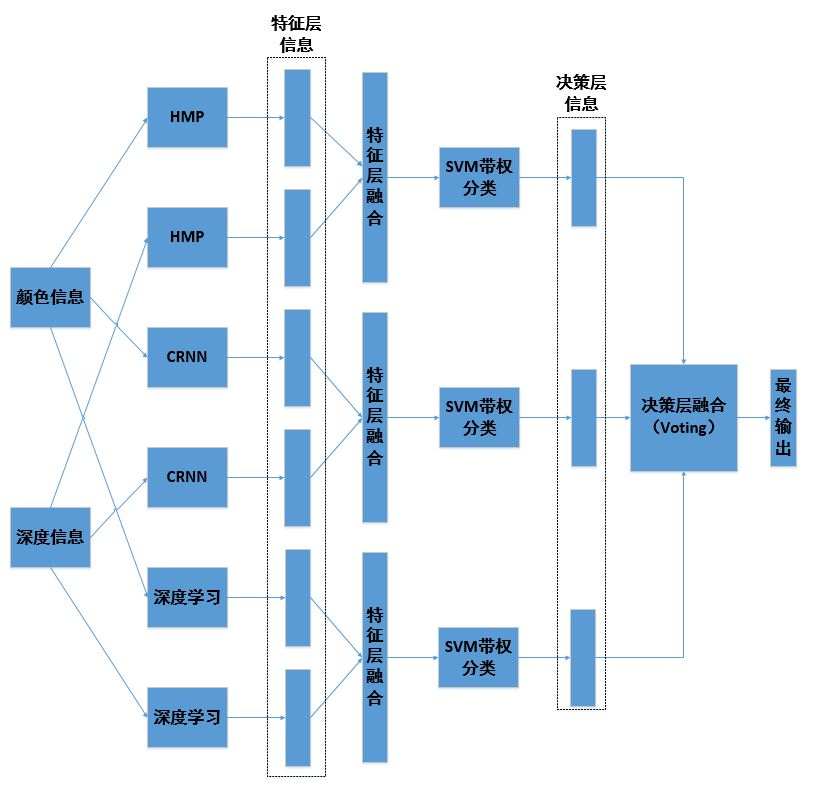
\includegraphics[width=0.9\textwidth]{workflow_general}
  \caption{综合分类模型工作流}
  \label{fig:workflow_general}
\end{figure}

在现有的方法中,传统词袋方法的识别精度不能尽如人意。而深度学习学习虽然准确率较高,但需要大规模数据库的支持。而我们提出的综合分类模型则结合了多种方法的优点:在没有大规模数据库支持时(即表~\ref{tab:cModelResult} 中的FS$^{1}$),深度学习表现一般,但有词袋模型作为准确率的支撑;在有大规模数据库或相关大规模数据库中预训练的模型时(即表~\ref{tab:cModelResult} 中的PM$^{2}$),则深度学习识别的准确率超过传统方法,对最终分类结果可以发挥极大的贡献。
最终模型的识别结果如表~\ref{tab:cModelResult} 所示。
注意由于综合模型中是三方融合,我们还尝试使用了多数投票(Majority Voting)作为融合策略,最终识别结果为91.3\%,略低于我们的带权投票。

\begin{table}[htbp]
  \centering
  \caption{综合模型实验结果}
  \label{tab:cModelResult}
  \begin{minipage}[t]{0.8\textwidth} 
    \begin{tabularx}{\linewidth}{|l|l|X|X|X|}
      \hline
      \multicolumn{2}{|c|}{\diagbox[width=7em]{方法}{模态}} & RGB & Depth & RGB \& Depth\\ \hline
      \multicolumn{2}{|c|}{CRNN}         & $81.7 \pm 1.4$ & $78.9 \pm 1.6$ & $87.6 \pm 1.2$ \\ \hline
      \multicolumn{2}{|c|}{HMP}          & $75.8 \pm 3.4$ & $78.4 \pm 1.9$ & $85.4 \pm 2.6$ \\ \hline
      \multicolumn{2}{|c|}{CRNN \& HMP}  & $83.1 \pm 2.6$ & $82.5 \pm 1.9$ & $89.6 \pm 2.1$ \\ \hline
      \multirow{2}*{深度学习} & FS$^{1}$ & $80.3 \pm 2.6$ & $70.7 \pm 2.3$ & $82.8 \pm 2.4$ \\ \cline{2-5}
                              & PM$^{2}$ & $85.5 \pm 1.5$ & $81.6 \pm 2.8$ & $90.3 \pm 1.8$ \\ \hline
      \multirow{2}*{综合模型} & FS$^{1}$ & $84.1 \pm 2.3$ & $81.9 \pm 2.5$ & $90.1 \pm 1.6$ \\ \cline{2-5}
                              & PM$^{2}$ & $86.9 \pm 1.3$ & $83.8 \pm 2.9$ & $91.6 \pm 1.2$ \\ \hline
    \end{tabularx}\\[2pt]
    \footnotesize
    本表展示的深度信息数据均是经过微调和DAN处理得到的结果,深度学习数据均是采用 fc6 单层信息得到的结果。且方法内均使用~\ref{subsec:fInMethod} 小节描述的特征层融合方法,方法间均使用~\ref{subsec:fBetweenMethod} 小节描述的决策层融合方法。\\
    1:不借助其他数据集从头训练(from scratch)\\
    2:使用在其他数据集上预训练的模型(pretrained model)
  \end{minipage}
\end{table}


各个类的分类准确率如图~\ref{fig:allacc} 所示,可见最终综合模型的百分之八十的类别分类准确率都在百分之九十以上,并且对于大部分类别,综合模型的分类准确率都高于三种方法单独的分类准确率。

不过如果我们重点看最分类准确率最低的十个类(如图~\ref{fig:10worstacc} 所示),可以发现,这些类别分类效果差一方面是因为数据本身问题——三种分类方法准确率都不高;另一方面也是由于分类融合策略在某些类别中被表现较差的方法“拖了后腿”,而没有发挥出表现好的类别的效果。这应该是我们下一步重点探讨的问题。

\begin{figure}[H] % use float package if you want it here
  \centering
  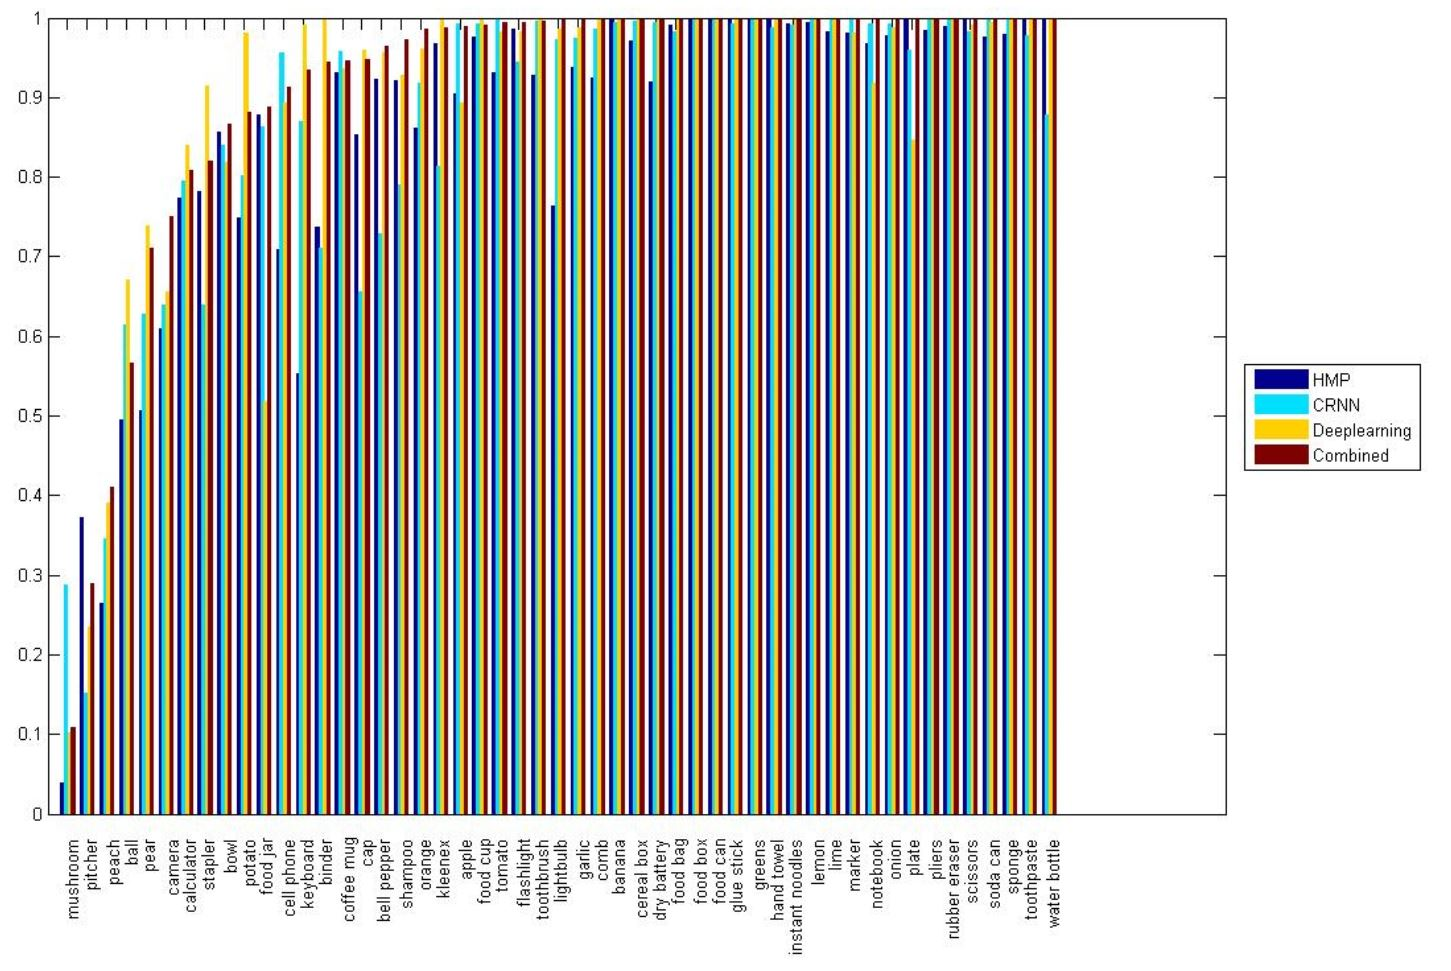
\includegraphics[width=0.95\textwidth]{allacc}
  \caption{分类准确率一览}
  \label{fig:allacc}
\end{figure}

\begin{figure}[H] % use float package if you want it here
  \centering
  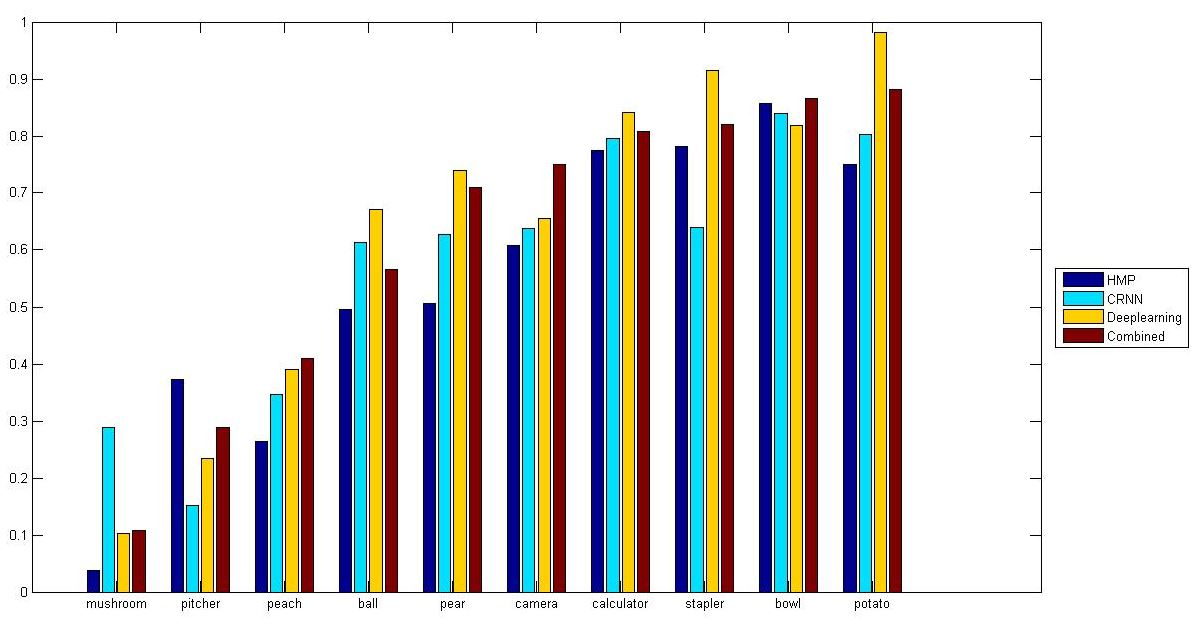
\includegraphics[width=0.95\textwidth]{10worstacc}
  \caption{分类准确率最低的十个类}
  \label{fig:10worstacc}
\end{figure}


\section{多模态识别程序}
\label{sec:demo}

我们按照~\ref{sec:comprehensiveModalResult} 节描述的综合模型实现了具有图形界面的多模态识别实例程序。

程序的流程图如~\ref{fig:workflow_demo} 所示,程序的界面如图~\ref{fig:demo} 所示。在程序开始时会自动载入训练好的 Model ,在识别时可以输入RGB图片和深度图片信息,并选择使用单模态或多模态分类器进行分类。具体分类效果由模型决定,在Qt程序中只做简单的预处理。

\begin{figure}[H] % use float package if you want it here
  \centering
  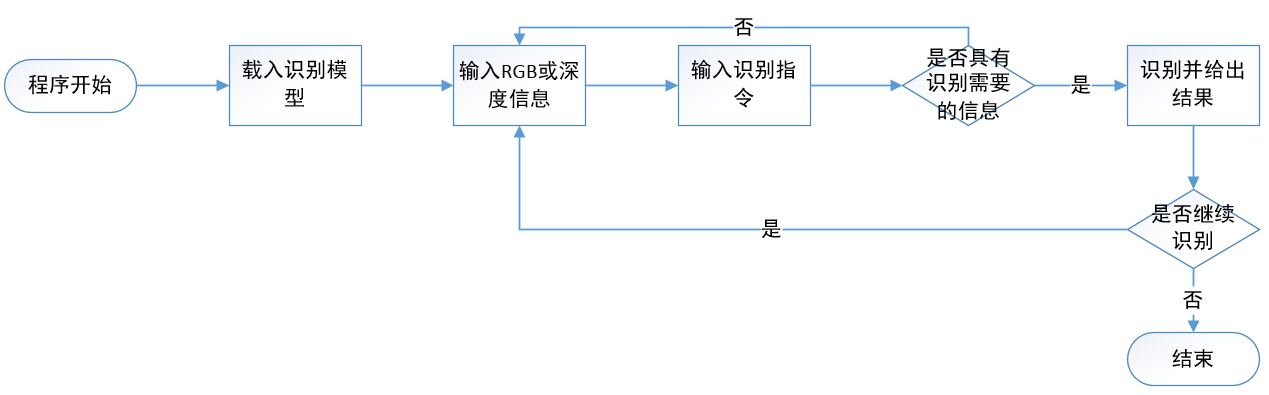
\includegraphics[width=0.95\textwidth]{workflow_demo}
  \caption{多模态识别程序流程图}
  \label{fig:workflow_demo}
\end{figure}

试验平台:
\begin{code}
Windows 8.1
Qt Creator 2.8.1
\end{code}

编译器:
\begin{code}
Qt5.1.1 (MSVC 2010, 32 bit)
GNU Make 3.82.90
Built for i686-w64-mingw32
\end{code}

\begin{figure}[H] % use float package if you want it here
  \centering
  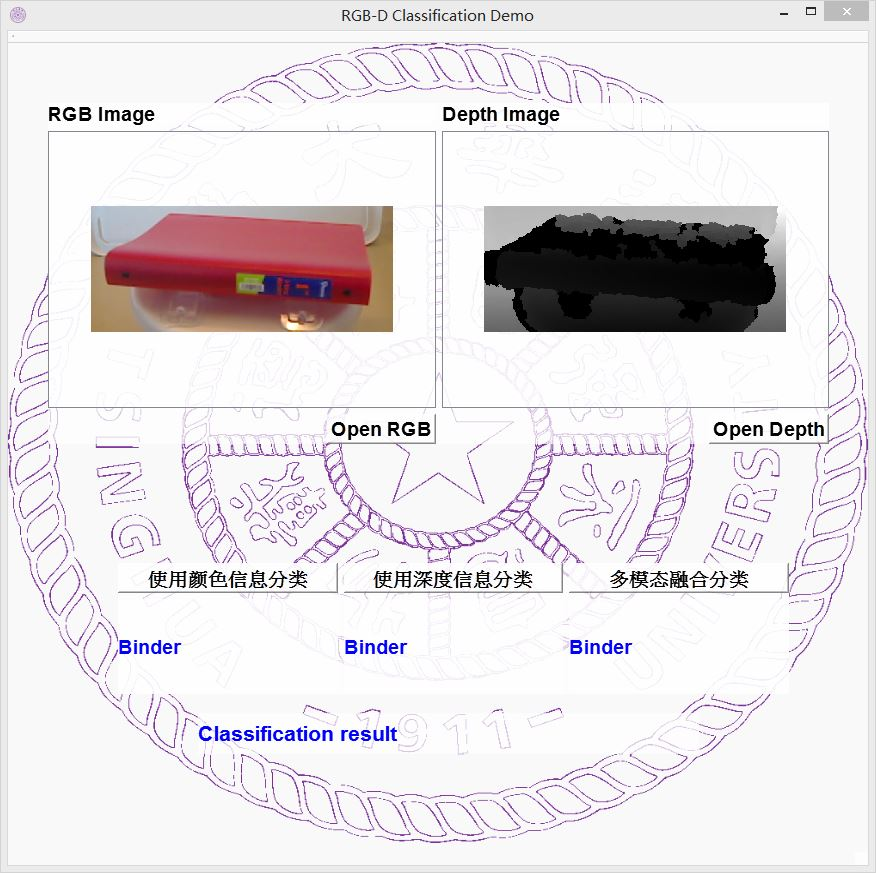
\includegraphics[width=0.95\textwidth]{demo}
  \caption{多模态识别程序界面}
  \label{fig:demo}
\end{figure}

% @Author: bo
% @Date:   2016-05-30 08:28:29
% @Last Modified by:   bo
% @Last Modified time: 2016-06-06 10:48:30

\chapter{总结与展望}
\label{cha:conclusion}

\section{本文总结}
\label{sec:conclusion}

本文研究了多方法多模态信息融合策略以及深度学习在多模态信息融合中的应用,具体的工作有:
\begin{enumerate}
  \item 首先,我们利用传统的分层匹配追踪,以及随机权值卷积递归神经网络来进行颜色和深度信息的提取和融合,并探究不同模态的信息之间的互补性。然后我们在这两种方法的基础上提出了一种决策层的信息融合策略,并探究不同方法之间的互补性。实验表明,不仅仅不同模态的信息之间具有互补性,不同信息提取方法之间也具有很强的互补性。将不同模态的信息或不同信息提取方法进行融合都可以使得我们对目标物体特征的感知变得更加全面,可以获得更好的识别效果。大量已有工作都是仅限于利用多传感器或不同模态之间的融合,而我们引入的不同方法之间融合的思路,可以进一步利用数据的互补性,弥补各个方法的不足。
  \item 其次,本文在传统信息提取方法之外还引入了深度学习方法。即使用八层的大型卷积神经网络在颜色信息和深度信息中分别进行深度学习,然后将相应的特征层信息提取出来,并进行模态之间的特征层信息融合,最终给出识别结果。此外,本文还提出了一种将深度信息转换为图片信息的正规化方法。这种方法对于深度信息的不同部分采用不同的正规化尺度,从而实现了既保留目标物体与背景之间的间隔,同时又保留目标物体之内形状变化信息的目的。实验证明,所提的深度信息正规化方法可以提升深度学习的识别准确率。
  \item 同时,为了解决深度学习中数据量不足的问题,我们使用了预先在海量图片数据集中训练过的模型来进行信息提取。而且由于已有模型是在颜色信息数据集中训练的,我们使用已有深度信息对其进行了微调,使它可以更好地适应深度信息的提取。试验证明,使用RGB图片预先训练的深度学习模型可以较好地识别颜色和深度信息。最后,我们基于以上研究提出了综合分层匹配追踪、随机权值递归神经网络以及深度学习三种方法的信息融合识别模型。实验证明,我们的融合模型可以提升识别的准确率和稳定性,并且降低了深度学习对于数据量的依赖。
\end{enumerate}

\section{未来工作展望}
\label{sec:future}

本文研究了多方法多模态信息融合策略,对不同层次的多种信息融合策略进行了较深入的探讨和实验,提高了分类的准确率和稳定性。不过仍有一些可以进一步完善的方向。具体有:
\begin{enumerate}
\item 进一步探究多模态信息融合策略。
在本文的探讨与实验中,我们完善了多模态信息融合方面的策略与方法。不过在实验中我们发现,多模态信息融合的潜力还有待开发,应用空间还很广阔。因此,进一步开发多模态信息融合的潜力,以便在各类机器人应用中发挥更大的效果是颇有意义的。
\item 探究深度学习在其他模态识别等任务中的应用。
我们知道传统深度学习需要的数据量是非常可观的,因而只在图像识别、分类、分割等应用中获得过较好的结果。但在本文中我们成功的将深度学习应用到了深度信息当中,尽管我们使用深度信息的数据规模并不是很大。这就为我们将深度学习的方法和模型应用到其他模态和领域开辟了道路。在本文中我们将只是将深度信息正规化为图片信息就可以使用预训练的模型取得较好的分类结果,下一步我们可以将其他模态的信息也编码为图片信息,并使用预训练的模型进行微调和分类。
\item 探究更多模态的融合。
本文只是将颜色信息和深度信息结合了起来,就获得了识别准确率和稳定性上的显著提升。然而现实中的信息模态远远不止这两种,而且有些模态与RGB-D的信息之间具有天然的更大的互补性。例如触觉信息和滑觉信息可以告诉我们目标物体的材质力学信息和摩擦力信息等等。而现实中的机器人操作往往是在错综复杂的环境中进行的,在机器人的感知和操作中考虑更多模态的融合,将会使机器人获得对环境的更加全面的认知,并作出更加智能的决策。
\end{enumerate}
% \chapter{带 English 的标题}
\label{cha:intro}

这是 \thuthesis{} 的示例文档,基本上覆盖了模板中所有格式的设置。建议大家在使用模
板之前,除了阅读《\thuthesis{}用户手册》,这个示例文档也最好能看一看。

小老鼠偷吃热凉粉;短长虫环绕矮高粱\footnote{韩愈(768-824),字退之,河南河阳(
  今河南孟县)人,自称郡望昌黎,世称韩昌黎。幼孤贫刻苦好学,德宗贞元八年进士。曾
  任监察御史,因上疏请免关中赋役,贬为阳山县令。后随宰相裴度平定淮西迁刑部侍郎,
  又因上表谏迎佛骨,贬潮州刺史。做过吏部侍郎,死谥文公,故世称韩吏部、韩文公。是
  唐代古文运动领袖,与柳宗元合称韩柳。诗力求险怪新奇,雄浑重气势。}。


\section{封面相关}
封面的例子请参看 cover.tex。主要符号表参看 denation.tex,附录和个人简历分别参看 appendix01.tex
和 resume.tex。里面的命令都很只管,一看即会\footnote{你说还是看不懂?怎么会呢?}。

\section{字体命令}
\label{sec:first}

苏轼(1037-1101),北宋文学家、书画家。字子瞻,号东坡居士,眉州眉山(今属四川)人
。苏洵子。嘉佑进士。神宗时曾任祠部员外郎,因反对王安石新法而求外职,任杭州通判,
知密州、徐州、湖州。后以作诗“谤讪朝廷”罪贬黄州。哲宗时任翰林学士,曾出知杭州、
颖州等,官至礼部尚书。后又贬谪惠州、儋州。北还后第二年病死常州。南宋时追谥文忠。
与父洵弟辙,合称“三苏”。在政治上属于旧党,但也有改革弊政的要求。其文汪洋恣肆,
明白畅达,为“唐宋八大家”之一。  其诗清新豪健,善用夸张比喻,在艺术表现方面独具
风格。少数诗篇也能反映民间疾苦,指责统治者的奢侈骄纵。词开豪放一派,对后代很有影
响。《念奴娇·赤壁怀古》、《水调歌头·丙辰中秋》传诵甚广。

{\kaishu 坡仙擅长行书、楷书,取法李邕、徐浩、颜真卿、杨凝式,而能自创新意。用笔丰腴
  跌宕,有天真烂漫之趣。与蔡襄、黄庭坚、米芾并称“宋四家”。能画竹,学文同,也喜
  作枯木怪石。论画主张“神似”,认为“论画以形似,见与儿童邻”;高度评价“诗中有
  画,画中有诗”的艺术造诣。诗文有《东坡七集》等。存世书迹有《答谢民师论文帖》、
  《祭黄几道文》、《前赤壁赋》、《黄州寒食诗帖》等。  画迹有《枯木怪石图》、《
  竹石图》等。}

{\fangsong 易与天地准,故能弥纶天地之道。仰以观於天文,俯以察於地理,是故知幽明之故。原
  始反终,故知死生之说。精气为物,游魂为变,是故知鬼神之情状。与天地相似,故不违。
  知周乎万物,而道济天下,故不过。旁行而不流,乐天知命,故不忧。安土敦乎仁,故
  能爱。范围天地之化而不过,曲成万物而不遗,通乎昼夜之道而知,故神无方而易无体。}

% 非本科生一般用不到幼圆与隶书字体。需要的同学请查看 ctex 文档。
{\ifcsname youyuan\endcsname\youyuan\else[无 \cs{youyuan} 字体。]\fi 有天地,然后
  万物生焉。盈天地之间者,唯万物,故受之以屯;屯者盈也,屯者物之始生也。物生必蒙,
  故受之以蒙;蒙者蒙也,物之穉也。物穉不可不养也,故受之以需;需者饮食之道也。饮
  食必有讼,故受之以讼。讼必有众起,故受之以师;师者众也。众必有所比,故受之以比;
  比者比也。比必有所畜也,故受之以小畜。物畜然后有礼,故受之以履。}

{\heiti 履而泰,然后安,故受之以泰;泰者通也。物不可以终通,故受之以否。物不可以终
  否,故受之以同人。与人同者,物必归焉,故受之以大有。有大者不可以盈,故受之以谦。
  有大而能谦,必豫,故受之以豫。豫必有随,故受之以随。以喜随人者,必有事,故受
  之以蛊;蛊者事也。}

{\ifcsname lishu\endcsname\lishu\else[无 \cs{lishu} 字体。]\fi 有事而后可大,故受
  之以临;临者大也。物大然后可观,故受之以观。可观而后有所合,故受之以噬嗑;嗑者
  合也。物不可以苟合而已,故受之以贲;贲者饰也。致饰然后亨,则尽矣,故受之以剥;
  剥者剥也。物不可以终尽,剥穷上反下,故受之以复。复则不妄矣,故受之以无妄。}

{\songti 有无妄然后可畜,故受之以大畜。物畜然后可养,故受之以颐;颐者养也。不养则不
  可动,故受之以大过。物不可以终过,故受之以坎;坎者陷也。陷必有所丽,故受之以
  离;离者丽也。}

\section{表格样本}
\label{chap1:sample:table} 

\subsection{基本表格}
\label{sec:basictable}

模板中关于表格的宏包有三个: \pkg{booktabs}、\pkg{array} 和
\pkg{longtabular},命令有一个 \cs{hlinewd}。三线表可以用 \pkg{booktabs}
提供的 \cs{toprule}、\cs{midrule} 和 \cs{bottomrule}。它们与
\pkg{longtable} 能很好的配合使用。如果表格比较简单的话可以直接用命令
\cs{hlinewd}\marg{width} 控制。
\begin{table}[htb]
  \centering
  \begin{minipage}[t]{0.8\linewidth} % 如果想在表格中使用脚注,minipage是个不错的办法
  \caption[模板文件]{模板文件。如果表格的标题很长,那么在表格索引中就会很不美
    观,所以要像 chapter 那样在前面用中括号写一个简短的标题。这个标题会出现在索
    引中。}
  \label{tab:template-files}
    \begin{tabularx}{\linewidth}{lX}
      \toprule[1.5pt]
      {\heiti 文件名} & {\heiti 描述} \\\midrule[1pt]
      thuthesis.ins & \LaTeX{} 安装文件,\textsc{DocStrip}\footnote{表格中的脚注} \\
      thuthesis.dtx & 所有的一切都在这里面\footnote{再来一个}。\\
      thuthesis.cls & 模板类文件。\\
      thuthesis.cfg & 模板配置文。cls 和 cfg 由前两个文件生成。\\
      thuthesis.bst    & 参考文献 BIB\TeX\ 样式文件。\\
      thuthesis.sty   & 常用的包和命令写在这里,减轻主文件的负担。\\
      \bottomrule[1.5pt]
    \end{tabularx}
  \end{minipage}
\end{table}

首先来看一个最简单的表格。表 \ref{tab:template-files} 列举了本模板主要文件及其功
能。请大家注意三线表中各条线对应的命令。这个例子还展示了如何在表格中正确使用脚注。
由于 \LaTeX{} 本身不支持在表格中使用 \cs{footnote},所以我们不得不将表格放在
小页中,而且最好将表格的宽度设置为小页的宽度,这样脚注看起来才更美观。

\subsection{复杂表格}
\label{sec:complicatedtable}

我们经常会在表格下方标注数据来源,或者对表格里面的条目进行解释。前面的脚注是一种
不错的方法,如果不喜欢脚注,可以在表格后面写注释,比如表~\ref{tab:tabexamp1}。
\begin{table}[htbp]
  \centering
  \caption{复杂表格示例 1}
  \label{tab:tabexamp1}
  \begin{minipage}[t]{0.8\textwidth} 
    \begin{tabularx}{\linewidth}{|l|X|X|X|X|}
      \hline
 \multirow{2}*{\diagbox[width=5em]{x}{y}} & \multicolumn{2}{c|}{First Half} & \multicolumn{2}{c|}{Second Half}\\\cline{2-5}
      & 1st Qtr &2nd Qtr&3rd Qtr&4th Qtr \\ \hline
      East$^{*}$ &   20.4&   27.4&   90&     20.4 \\
      West$^{**}$ &   30.6 &   38.6 &   34.6 &  31.6 \\ \hline
    \end{tabularx}\\[2pt]
    \footnotesize 注:数据来源《\thuthesis{} 使用手册》。\\
    *:东部\\
    **:西部
  \end{minipage}
\end{table}

此外,表~\ref{tab:tabexamp1} 同时还演示了另外两个功能:1)通过 \pkg{tabularx} 的
 \texttt{|X|} 扩展实现表格自动放大;2)通过命令 \cs{diagbox} 在表头部分
插入反斜线。

为了使我们的例子更接近实际情况,我会在必要的时候插入一些“无关”文字,以免太多图
表同时出现,导致排版效果不太理想。第一个出场的当然是我的最爱:风流潇洒、骏马绝尘、
健笔凌云的{\heiti 李太白}了。

李白,字太白,陇西成纪人。凉武昭王暠九世孙。或曰山东人,或曰蜀人。白少有逸才,志
气宏放,飘然有超世之心。初隐岷山,益州长史苏颋见而异之,曰:“是子天才英特,可比
相如。”天宝初,至长安,往见贺知章。知章见其文,叹曰:“子谪仙人也。”言于明皇,
召见金銮殿,奏颂一篇。帝赐食,亲为调羹,有诏供奉翰林。白犹与酒徒饮于市,帝坐沉香
亭子,意有所感,欲得白为乐章,召入,而白已醉。左右以水颒面,稍解,援笔成文,婉丽
精切。帝爱其才,数宴见。白常侍帝,醉,使高力士脱靴。力士素贵,耻之,摘其诗以激杨
贵妃。帝欲官白,妃辄沮止。白自知不为亲近所容,恳求还山。帝赐金放还。乃浪迹江湖,
终日沉饮。永王璘都督江陵,辟为僚佐。璘谋乱,兵败,白坐长流夜郎,会赦得还。族人阳
冰为当涂令,白往依之。代宗立,以左拾遗召,而白已卒。文宗时,诏以白歌诗、裴旻剑舞、
张旭草书为三绝云。集三十卷。今编诗二十五卷。\hfill —— 《全唐诗》诗人小传

浮动体的并排放置一般有两种情况:1)二者没有关系,为两个独立的浮动体;2)二者隶属
于同一个浮动体。对表格来说并排表格既可以像图~\ref{tab:parallel1}、图~\ref{tab:parallel2} 
使用小页环境,也可以如图~\ref{tab:subtable} 使用子表格来做。图的例子参见第~\ref{sec:multifig} 节。

\begin{table}[htbp]
\noindent\begin{minipage}{0.5\textwidth}
\centering
\caption{第一个并排子表格}
\label{tab:parallel1}
\begin{tabular}{p{2cm}p{2cm}}
\toprule[1.5pt]
111 & 222 \\\midrule[1pt]
222 & 333 \\\bottomrule[1.5pt]
\end{tabular}
\end{minipage}%
\begin{minipage}{0.5\textwidth}
\centering
\caption{第二个并排子表格}
\label{tab:parallel2}
\begin{tabular}{p{2cm}p{2cm}}
\toprule[1.5pt]
111 & 222 \\\midrule[1pt]
222 & 333 \\\bottomrule[1.5pt]
\end{tabular}
\end{minipage}
\end{table}

然后就是忧国忧民,诗家楷模杜工部了。杜甫,字子美,其先襄阳人,曾祖依艺为巩令,因
居巩。甫天宝初应进士,不第。后献《三大礼赋》,明皇奇之,召试文章,授京兆府兵曹参
军。安禄山陷京师,肃宗即位灵武,甫自贼中遁赴行在,拜左拾遗。以论救房琯,出为华州
司功参军。关辅饥乱,寓居同州同谷县,身自负薪采梠,餔糒不给。久之,召补京兆府功曹,
道阻不赴。严武镇成都,奏为参谋、检校工部员外郎,赐绯。武与甫世旧,待遇甚厚。乃于
成都浣花里种竹植树,枕江结庐,纵酒啸歌其中。武卒,甫无所依,乃之东蜀就高適。既至
而適卒。是岁,蜀帅相攻杀,蜀大扰。甫携家避乱荆楚,扁舟下峡,未维舟而江陵亦乱。乃
溯沿湘流,游衡山,寓居耒阳。卒年五十九。元和中,归葬偃师首阳山,元稹志其墓。天宝
间,甫与李白齐名,时称李杜。然元稹之言曰:“李白壮浪纵恣,摆去拘束,诚亦差肩子美
矣。至若铺陈终始,排比声韵,大或千言,次犹数百,词气豪迈,而风调清深,属对律切,
而脱弃凡近,则李尚不能历其藩翰,况堂奥乎。”白居易亦云:“杜诗贯穿古今,  尽工尽
善,殆过于李。”元、白之论如此。盖其出处劳佚,喜乐悲愤,好贤恶恶,一见之于诗。而
又以忠君忧国、伤时念乱为本旨。读其诗可以知其世,故当时谓之“诗史”。旧集诗文共六
十卷,今编诗十九卷。

\begin{table}[htbp]
\centering
\caption{并排子表格}
\label{tab:subtable}
\subcaptionbox{第一个子表格}
{
\begin{tabular}{p{2cm}p{2cm}}
\toprule[1.5pt]
111 & 222 \\\midrule[1pt]
222 & 333 \\\bottomrule[1.5pt]
\end{tabular}
}
\hskip2cm
\subcaptionbox{第二个子表格}
{
\begin{tabular}{p{2cm}p{2cm}}
\toprule[1.5pt]
111 & 222 \\\midrule[1pt]
222 & 333 \\\bottomrule[1.5pt]
\end{tabular}
}
\end{table}

不可否认 \LaTeX{} 的表格功能没有想象中的那么强大,不过只要足够认真,足够细致,
同样可以排出来非常复杂非常漂亮的表格。请参看表~\ref{tab:tabexamp2}。
\begin{table}[htbp]
  \centering\dawu[1.3]
  \caption{复杂表格示例 2}
  \label{tab:tabexamp2}
  \begin{tabular}[c]{|m{1.5cm}|c|c|c|c|c|c|}\hline
    \multicolumn{2}{|c|}{Network Topology} & \# of nodes & 
    \multicolumn{3}{c|}{\# of clients} & Server \\\hline
    GT-ITM & Waxman Transit-Stub & 600 &
    \multirow{2}{2em}{2\%}& 
    \multirow{2}{2em}{10\%}& 
    \multirow{2}{2em}{50\%}& 
    \multirow{2}{1.2in}{Max. Connectivity}\\\cline{1-3}
    \multicolumn{2}{|c|}{Inet-2.1} & 6000 & & & &\\\hline
    \multirow{2}{1.5cm}{Xue} & Rui  & Ni &\multicolumn{4}{c|}{\multirow{2}*{\thuthesis}}\\\cline{2-3}
    & \multicolumn{2}{c|}{ABCDEF} &\multicolumn{4}{c|}{} \\\hline
\end{tabular}
\end{table}

最后就是清新飘逸、文约意赅、空谷绝响的王大侠了。王维,字摩诘,河东人。工书画,与
弟缙俱有俊才。开元九年,进士擢第,调太乐丞。坐累为济州司仓参军,历右拾遗、监察御
史、左补阙、库部郎中,拜吏部郎中。天宝末,为给事中。安禄山陷两都,维为贼所得,服
药阳喑,拘于菩提寺。禄山宴凝碧池,维潜赋诗悲悼,闻于行在。贼平,陷贼官三等定罪,
特原之,责授太子中允,迁中庶子、中书舍人。复拜给事中,转尚书右丞。维以诗名盛于开
元、天宝间,宁薛诸王驸马豪贵之门,无不拂席迎之。得宋之问辋川别墅,山水绝胜,与道
友裴迪,浮舟往来,弹琴赋诗,啸咏终日。笃于奉佛,晚年长斋禅诵。一日,忽索笔作书
数纸,别弟缙及平生亲故,舍笔而卒。赠秘书监。宝应中,代宗问缙:“朕常于诸王坐闻维
乐章,今存几何?”缙集诗六卷,文四卷,表上之。敕答云,卿伯氏位列先朝,名高希代。
抗行周雅,长揖楚辞。诗家者流,时论归美。克成编录,叹息良深。殷璠谓维诗词秀调雅,
意新理惬。在泉成珠,著壁成绘。苏轼亦云:“维诗中有画,画中有诗也。”今编诗四卷。

要想用好论文模板还是得提前学习一些 \TeX/\LaTeX{}的相关知识,具备一些基本能力,掌
握一些常见技巧,否则一旦遇到问题还真是比较麻烦。我们见过很多这样的同学,一直以来
都是使用 Word 等字处理工具,以为 \LaTeX{}模板的用法也应该类似,所以就沿袭同样的思
路来对待这种所见非所得的排版工具,结果被折腾的焦头烂额,疲惫不堪。

如果您要排版的表格长度超过一页,那么推荐使用 \pkg{longtable} 或者 \pkg{supertabular}
宏包,模板对 \pkg{longtable} 进行了相应的设置,所以用起来可能简单一些。
表~\ref{tab:performance} 就是 \pkg{longtable} 的简单示例。
\begin{longtable}[c]{c*{6}{r}}
\caption{实验数据}\label{tab:performance}\\
\toprule[1.5pt]
 测试程序 & \multicolumn{1}{c}{正常运行} & \multicolumn{1}{c}{同步} & \multicolumn{1}{c}{检查点} & \multicolumn{1}{c}{卷回恢复}
& \multicolumn{1}{c}{进程迁移} & \multicolumn{1}{c}{检查点} \\
& \multicolumn{1}{c}{时间 (s)}& \multicolumn{1}{c}{时间 (s)}&
\multicolumn{1}{c}{时间 (s)}& \multicolumn{1}{c}{时间 (s)}& \multicolumn{1}{c}{
  时间 (s)}&  文件(KB)\\\midrule[1pt]
\endfirsthead
\multicolumn{7}{c}{续表~\thetable\hskip1em 实验数据}\\
\toprule[1.5pt]
 测试程序 & \multicolumn{1}{c}{正常运行} & \multicolumn{1}{c}{同步} & \multicolumn{1}{c}{检查点} & \multicolumn{1}{c}{卷回恢复}
& \multicolumn{1}{c}{进程迁移} & \multicolumn{1}{c}{检查点} \\
& \multicolumn{1}{c}{时间 (s)}& \multicolumn{1}{c}{时间 (s)}&
\multicolumn{1}{c}{时间 (s)}& \multicolumn{1}{c}{时间 (s)}& \multicolumn{1}{c}{
  时间 (s)}&  文件(KB)\\\midrule[1pt]
\endhead
\hline
\multicolumn{7}{r}{续下页}
\endfoot
\endlastfoot
CG.A.2 & 23.05 & 0.002 & 0.116 & 0.035 & 0.589 & 32491 \\
CG.A.4 & 15.06 & 0.003 & 0.067 & 0.021 & 0.351 & 18211 \\
CG.A.8 & 13.38 & 0.004 & 0.072 & 0.023 & 0.210 & 9890 \\
CG.B.2 & 867.45 & 0.002 & 0.864 & 0.232 & 3.256 & 228562 \\
CG.B.4 & 501.61 & 0.003 & 0.438 & 0.136 & 2.075 & 123862 \\
CG.B.8 & 384.65 & 0.004 & 0.457 & 0.108 & 1.235 & 63777 \\
MG.A.2 & 112.27 & 0.002 & 0.846 & 0.237 & 3.930 & 236473 \\
MG.A.4 & 59.84 & 0.003 & 0.442 & 0.128 & 2.070 & 123875 \\
MG.A.8 & 31.38 & 0.003 & 0.476 & 0.114 & 1.041 & 60627 \\
MG.B.2 & 526.28 & 0.002 & 0.821 & 0.238 & 4.176 & 236635 \\
MG.B.4 & 280.11 & 0.003 & 0.432 & 0.130 & 1.706 & 123793 \\
MG.B.8 & 148.29 & 0.003 & 0.442 & 0.116 & 0.893 & 60600 \\
LU.A.2 & 2116.54 & 0.002 & 0.110 & 0.030 & 0.532 & 28754 \\
LU.A.4 & 1102.50 & 0.002 & 0.069 & 0.017 & 0.255 & 14915 \\
LU.A.8 & 574.47 & 0.003 & 0.067 & 0.016 & 0.192 & 8655 \\
LU.B.2 & 9712.87 & 0.002 & 0.357 & 0.104 & 1.734 & 101975 \\
LU.B.4 & 4757.80 & 0.003 & 0.190 & 0.056 & 0.808 & 53522 \\
LU.B.8 & 2444.05 & 0.004 & 0.222 & 0.057 & 0.548 & 30134 \\
EP.A.2 & 123.81 & 0.002 & 0.010 & 0.003 & 0.074 & 1834 \\
EP.A.4 & 61.92 & 0.003 & 0.011 & 0.004 & 0.073 & 1743 \\
EP.A.8 & 31.06 & 0.004 & 0.017 & 0.005 & 0.073 & 1661 \\
EP.B.2 & 495.49 & 0.001 & 0.009 & 0.003 & 0.196 & 2011 \\
EP.B.4 & 247.69 & 0.002 & 0.012 & 0.004 & 0.122 & 1663 \\
EP.B.8 & 126.74 & 0.003 & 0.017 & 0.005 & 0.083 & 1656 \\
\bottomrule[1.5pt]
\end{longtable}

\subsection{其它}
\label{sec:tableother}
如果不想让某个表格或者图片出现在索引里面,请使用命令 \cs{caption*}。
这个命令不会给表格编号,也就是出来的只有标题文字而没有“表~XX”,“图~XX”,否则
索引里面序号不连续就显得不伦不类,这也是 \LaTeX{} 里星号命令默认的规则。

有这种需求的多是本科同学的英文资料翻译部分,如果觉得附录中英文原文中的表格和图
片显示成“表”和“图”不协调的话,一个很好的办法就是用 \cs{caption*},参数
随便自己写,比如不守规矩的表~1.111 和图~1.111 能满足这种特殊需要(可以参看附录部
分)。
\begin{table}[ht]
  \begin{minipage}{0.4\linewidth}
    \centering
    \caption*{表~1.111\quad 这是一个手动编号,不出现在索引中的表格。}
    \label{tab:badtabular}
      \framebox(150,50)[c]{\thuthesis}
  \end{minipage}%
  \hfill%
  \begin{minipage}{0.4\linewidth}
    \centering
    \caption*{Figure~1.111\quad 这是一个手动编号,不出现在索引中的图。}
    \label{tab:badfigure}
    \framebox(150,50)[c]{薛瑞尼}
  \end{minipage}
\end{table}

如果的确想让它编号,但又不想让它出现在索引中的话,目前模板上不支持。

最后,虽然大家不一定会独立使用小页,但是关于小页中的脚注还是有必要提一下。请看下
面的例子。

\begin{minipage}[t]{\linewidth-2\parindent}
  柳宗元,字子厚(773-819),河东(今永济县)人\footnote{山西永济水饺。},是唐代
  杰出的文学家,哲学家,同时也是一位政治改革家。与韩愈共同倡导唐代古文运动,并称
  韩柳\footnote{唐宋八大家之首二位。}。
\end{minipage}

唐朝安史之乱后,宦官专权,藩镇割据,土地兼并日渐严重,社会生产破坏严重,民不聊生。柳宗
元对这种社会现实极为不满,他积极参加了王叔文领导的“永济革新”,并成为这一
运动的中坚人物。他们革除弊政,打击权奸,触犯了宦官和官僚贵族利益,在他们的联合反
扑下,改革失败了,柳宗元被贬为永州司马。

\section{定理环境}
\label{sec:theorem}

给大家演示一下各种和证明有关的环境:

\begin{assumption}
待月西厢下,迎风户半开;隔墙花影动,疑是玉人来。
\begin{eqnarray}
  \label{eq:eqnxmp}
  c & = & a^2 - b^2\\
    & = & (a+b)(a-b)
\end{eqnarray}
\end{assumption}

千辛万苦,历尽艰难,得有今日。然相从数千里,未曾哀戚。今将渡江,方图百年欢笑,如
何反起悲伤?(引自《杜十娘怒沉百宝箱》)

\begin{definition}
子曰:「道千乘之国,敬事而信,节用而爱人,使民以时。」
\end{definition}

千古第一定义!问世间、情为何物,只教生死相许?天南地北双飞客,老翅几回寒暑。欢乐趣,离别苦,就中更有痴儿女。
君应有语,渺万里层云,千山暮雪,只影向谁去?

横汾路,寂寞当年箫鼓,荒烟依旧平楚。招魂楚些何嗟及,山鬼暗谛风雨。天也妒,未信与,莺儿燕子俱黄土。
千秋万古,为留待骚人,狂歌痛饮,来访雁丘处。

\begin{proposition}
 曾子曰:「吾日三省吾身 —— 为人谋而不忠乎?与朋友交而不信乎?传不习乎?」
\end{proposition}

多么凄美的命题啊!其日牛马嘶,新妇入青庐,奄奄黄昏后,寂寂人定初,我命绝今日,
魂去尸长留,揽裙脱丝履,举身赴清池,府吏闻此事,心知长别离,徘徊庭树下,自挂东南
枝。

\begin{remark}
天不言自高,水不言自流。
\begin{gather*}
\begin{split} 
\varphi(x,z)
&=z-\gamma_{10}x-\gamma_{mn}x^mz^n\\
&=z-Mr^{-1}x-Mr^{-(m+n)}x^mz^n
\end{split}\\[6pt]
\begin{align} \zeta^0&=(\xi^0)^2,\\
\zeta^1 &=\xi^0\xi^1,\\
\zeta^2 &=(\xi^1)^2,
\end{align}
\end{gather*}
\end{remark}

天尊地卑,乾坤定矣。卑高以陈,贵贱位矣。 动静有常,刚柔断矣。方以类聚,物以群分,
吉凶生矣。在天成象,在地成形,变化见矣。鼓之以雷霆,润之以风雨,日月运行,一寒一
暑,乾道成男,坤道成女。乾知大始,坤作成物。乾以易知,坤以简能。易则易知,简则易
从。易知则有亲,易从则有功。有亲则可久,有功则可大。可久则贤人之德,可大则贤人之
业。易简,而天下矣之理矣;天下之理得,而成位乎其中矣。

\begin{axiom}
两点间直线段距离最短。  
\begin{align}
x&\equiv y+1\pmod{m^2}\\
x&\equiv y+1\mod{m^2}\\
x&\equiv y+1\pod{m^2}
\end{align}
\end{axiom}

《彖曰》:大哉乾元,万物资始,乃统天。云行雨施,品物流形。大明始终,六位时成,时
乘六龙以御天。乾道变化,各正性命,保合大和,乃利贞。首出庶物,万国咸宁。

《象曰》:天行健,君子以自强不息。潜龙勿用,阳在下也。见龙再田,德施普也。终日乾
乾,反复道也。或跃在渊,进无咎也。飞龙在天,大人造也。亢龙有悔,盈不可久也。用九,
天德不可为首也。   

\begin{lemma}
《猫和老鼠》是我最爱看的动画片。
\begin{multline*}%\tag*{[a]} % 这个不出现在索引中
\int_a^b\biggl\{\int_a^b[f(x)^2g(y)^2+f(y)^2g(x)^2]
 -2f(x)g(x)f(y)g(y)\,dx\biggr\}\,dy \\
 =\int_a^b\biggl\{g(y)^2\int_a^bf^2+f(y)^2
  \int_a^b g^2-2f(y)g(y)\int_a^b fg\biggr\}\,dy
\end{multline*}
\end{lemma}

行行重行行,与君生别离。相去万余里,各在天一涯。道路阻且长,会面安可知。胡马依北
风,越鸟巢南枝。相去日已远,衣带日已缓。浮云蔽白日,游子不顾返。思君令人老,岁月
忽已晚。  弃捐勿复道,努力加餐饭。

\begin{theorem}\label{the:theorem1}
犯我强汉者,虽远必诛\hfill —— 陈汤(汉)
\end{theorem}
\begin{subequations}
\begin{align}
y & = 1 \\
y & = 0
\end{align}
\end{subequations}
道可道,非常道。名可名,非常名。无名天地之始;有名万物之母。故常无,欲以观其妙;
常有,欲以观其徼。此两者,同出而异名,同谓之玄。玄之又玄,众妙之门。上善若水。水
善利万物而不争,处众人之所恶,故几于道。曲则全,枉则直,洼则盈,敝则新,少则多,
多则惑。人法地,地法天,天法道,道法自然。知人者智,自知者明。胜人者有力,自胜
者强。知足者富。强行者有志。不失其所者久。死而不亡者寿。

\begin{proof}
燕赵古称多感慨悲歌之士。董生举进士,连不得志于有司,怀抱利器,郁郁适兹土,吾
知其必有合也。董生勉乎哉?

夫以子之不遇时,苟慕义强仁者,皆爱惜焉,矧燕、赵之士出乎其性者哉!然吾尝闻
风俗与化移易,吾恶知其今不异于古所云邪?聊以吾子之行卜之也。董生勉乎哉?

吾因子有所感矣。为我吊望诸君之墓,而观于其市,复有昔时屠狗者乎?为我谢
曰:“明天子在上,可以出而仕矣!” \hfill —— 韩愈《送董邵南序》
\end{proof}

\begin{corollary}
  四川话配音的《猫和老鼠》是世界上最好看最好听最有趣的动画片。
\begin{alignat}{3}
V_i & =v_i - q_i v_j, & \qquad X_i & = x_i - q_i x_j,
 & \qquad U_i & = u_i,
 \qquad \text{for $i\ne j$;}\label{eq:B}\\
V_j & = v_j, & \qquad X_j & = x_j,
  & \qquad U_j & u_j + \sum_{i\ne j} q_i u_i.
\end{alignat}
\end{corollary}

迢迢牵牛星,皎皎河汉女。
纤纤擢素手,札札弄机杼。
终日不成章,泣涕零如雨。
河汉清且浅,相去复几许。
盈盈一水间,脉脉不得语。

\begin{example}
  大家来看这个例子。
\begin{equation}
\label{ktc}
\left\{\begin{array}{l}
\nabla f({\mbox{\boldmath $x$}}^*)-\sum\limits_{j=1}^p\lambda_j\nabla g_j({\mbox{\boldmath $x$}}^*)=0\\[0.3cm]
\lambda_jg_j({\mbox{\boldmath $x$}}^*)=0,\quad j=1,2,\cdots,p\\[0.2cm]
\lambda_j\ge 0,\quad j=1,2,\cdots,p.
\end{array}\right.
\end{equation}
\end{example}

\begin{exercise}
  清列出 Andrew S. Tanenbaum 和 W. Richard Stevens 的所有著作。
\end{exercise}

\begin{conjecture} \textit{Poincare Conjecture} If in a closed three-dimensional
  space, any closed curves can shrink to a point continuously, this space can be
  deformed to a sphere.
\end{conjecture}

\begin{problem}
 回答还是不回答,是个问题。 
\end{problem}

如何引用定理~\ref{the:theorem1} 呢?加上 \cs{label} 使用 \cs{ref} 即可。妾发
初覆额,折花门前剧。郎骑竹马来,绕床弄青梅。同居长干里,两小无嫌猜。 十四为君妇,
羞颜未尝开。低头向暗壁,千唤不一回。十五始展眉,愿同尘与灰。常存抱柱信,岂上望夫
台。 十六君远行,瞿塘滟滪堆。五月不可触,猿声天上哀。门前迟行迹,一一生绿苔。苔深
不能扫,落叶秋风早。八月蝴蝶来,双飞西园草。感此伤妾心,坐愁红颜老。

\section{参考文献}
\label{sec:bib}
当然参考文献可以直接写 \cs{bibitem},虽然费点功夫,但是好控制,各种格式可以自己随意改
写。

本模板推荐使用 BIB\TeX,样式文件为 \texttt{thuthesis.bst},基本符合学校的参考文献格
式(如专利等引用未加详细测试)。看看这个例子,关于书的~\cite{tex, companion,
  ColdSources},还有这些~\cite{Krasnogor2004e, clzs, zjsw},关于杂志
的~\cite{ELIDRISSI94, MELLINGER96, SHELL02},硕士论文~\cite{zhubajie,
  metamori2004},博士论文~\cite{shaheshang, FistSystem01},标准文
件~\cite{IEEE-1363},会议论文~\cite{DPMG,kocher99},技术报告~\cite{NPB2},电子文
献~\cite{chuban2001,oclc2000}。中文参考文献~\cite{cnarticle}应增
加 \texttt{lang=``zh''} 字段,以便进行相应处理。另外,本模板对中文文
献~\cite{cnproceed}的支持并不是十全十美,如果有不如意的地方,请手动修
改 \texttt{bbl} 文件。

有时候不想要上标,那么可以这样~\inlinecite{shaheshang},这个非常重要。

有时候一些参考文献没有纸质出处,需要标注 URL。缺省情况下,URL 不会在连字符处断行,
这可能使得用连字符代替空格的网址分行很难看。如果需要,可以将模板类文件中
\begin{verbatim}
\RequirePackage{hyperref}
\end{verbatim}
一行改为:
\begin{verbatim}
\PassOptionsToPackage{hyphens}{url}
\RequirePackage{hyperref}
\end{verbatim}
使得连字符处可以断行。更多设置可以参考 \texttt{url} 宏包文档。

\section{公式}
\label{sec:equation}
贝叶斯公式如式~(\ref{equ:chap1:bayes}),其中 $p(y|\mathbf{x})$ 为后验;
$p(\mathbf{x})$ 为先验;分母 $p(\mathbf{x})$ 为归一化因子。
\begin{equation}
\label{equ:chap1:bayes}
p(y|\mathbf{x}) = \frac{p(\mathbf{x},y)}{p(\mathbf{x})}=
\frac{p(\mathbf{x}|y)p(y)}{p(\mathbf{x})} 
\end{equation}

论文里面公式越多,\TeX{} 就越 happy。再看一个 \pkg{amsmath} 的例子:
\newcommand{\envert}[1]{\left\lvert#1\right\rvert} 
\begin{equation}\label{detK2}
\det\mathbf{K}(t=1,t_1,\dots,t_n)=\sum_{I\in\mathbf{n}}(-1)^{\envert{I}}
\prod_{i\in I}t_i\prod_{j\in I}(D_j+\lambda_jt_j)\det\mathbf{A}
^{(\lambda)}(\overline{I}|\overline{I})=0.
\end{equation} 

前面定理示例部分列举了很多公式环境,可以说把常见的情况都覆盖了,大家在写公式的时
候一定要好好看 \pkg{amsmath} 的文档,并参考模板中的用法:
\begin{multline*}%\tag{[b]} % 这个出现在索引中的
\int_a^b\biggl\{\int_a^b[f(x)^2g(y)^2+f(y)^2g(x)^2]
 -2f(x)g(x)f(y)g(y)\,dx\biggr\}\,dy \\
 =\int_a^b\biggl\{g(y)^2\int_a^bf^2+f(y)^2
  \int_a^b g^2-2f(y)g(y)\int_a^b fg\biggr\}\,dy
\end{multline*}

其实还可以看看这个多级规划:
\begin{equation}\label{bilevel}
\left\{\begin{array}{l}
\max\limits_{{\mbox{\footnotesize\boldmath $x$}}} F(x,y_1^*,y_2^*,\cdots,y_m^*)\\[0.2cm]
\mbox{subject to:}\\[0.1cm]
\qquad G(x)\le 0\\[0.1cm]
\qquad(y_1^*,y_2^*,\cdots,y_m^*)\mbox{ solves problems }(i=1,2,\cdots,m)\\[0.1cm]
\qquad\left\{\begin{array}{l}
    \max\limits_{{\mbox{\footnotesize\boldmath $y_i$}}}f_i(x,y_1,y_2,\cdots,y_m)\\[0.2cm]
    \mbox{subject to:}\\[0.1cm]
    \qquad g_i(x,y_1,y_2,\cdots,y_m)\le 0.
    \end{array}\right.
\end{array}\right.
\end{equation}
这些跟规划相关的公式都来自于刘宝碇老师《不确定规划》的课件。

% \chapter{中华人民共和国}
\label{cha:china}

\section{其它例子}
\label{sec:other}

在第~\ref{cha:intro} 章中我们学习了贝叶斯公式~(\ref{equ:chap1:bayes}),这里我们复
习一下:
\begin{equation}
\label{equ:chap2:bayes}
p(y|\mathbf{x}) = \frac{p(\mathbf{x},y)}{p(\mathbf{x})}=
\frac{p(\mathbf{x}|y)p(y)}{p(\mathbf{x})}
\end{equation}

\subsection{绘图}
\label{sec:draw}

本模板不再预先装载任何绘图包(如 \pkg{pstricks,pgf} 等),完全由用户来决定。
个人觉得 \pkg{pgf} 不错,不依赖于 Postscript。此外还有很多针对 \LaTeX{} 的
 GUI 作图工具,如 XFig(jFig), WinFig, Tpx, Ipe, Dia, Inkscape, LaTeXPiX,
jPicEdt, jaxdraw 等等。

\subsection{插图}
\label{sec:graphs}

强烈推荐《\LaTeXe\ 插图指南》!关于子图形的使用细节请参看 \pkg{subcaption} 宏包的说明文档。

\subsubsection{一个图形}
\label{sec:onefig}
一般图形都是处在浮动环境中。之所以称为浮动是指最终排版效果图形的位置不一定与源文
件中的位置对应\footnote{This is not a bug, but a feature of \LaTeX!},这也是刚使
用 \LaTeX{} 同学可能遇到的问题。如果要强制固定浮动图形的位置,请使用 \pkg{float} 宏包,
它提供了 \texttt{[H]} 参数,比如图~\ref{fig:xfig1}。
\begin{figure}[H] % use float package if you want it here
  \centering
  
\includegraphics{thu-whole-logo}
  \caption{利用 Xfig 制图}
  \label{fig:xfig1}
\end{figure}

大学之道,在明明德,在亲民,在止于至善。知止而后有定;定而后能静;静而后能安;安
而后能虑;虑而后能得。物有本末,事有终始。知所先后,则近道矣。古之欲明明德于天
下者,先治其国;欲治其国者,先齐其家;欲齐其家者,先修其身;欲修其身者,先正其心;
欲正其心者,先诚其意;欲诚其意者,先致其知;致知在格物。物格而后知至;知至而后
意诚;意诚而后心正;心正而后身 修;身修而后家齐;家齐而后国治;国治而后天下
平。自天子以至于庶人,壹是皆以修身为本。其本乱而未治者 否矣。其所厚者薄,而其所
薄者厚,未之有也!

\hfill —— 《大学》


\subsubsection{多个图形}
\label{sec:multifig}

如果多个图形相互独立,并不共用一个图形计数器,那么
用 \texttt{minipage} 或者\texttt{parbox} 就可以。否则,请参看
图~\ref{fig:big1-subcaptionbox},它包含两个小图,分别是图~\ref{fig:subfig1}和
图~\ref{fig:subfig2}。推荐使用\cs{subcaptionbox},因为可以像
图~\ref{fig:big1-subcaptionbox} 那样对齐子图的标题,也可以使
用\pkg{subcaption}宏包的\cs{subcaption}(放在 minipage中,用法同\cs{caption})
或是 \pkg{subfigure} 、 \pkg{subtable}环境,像图~\ref{fig:big1-subfigure},
不要再用 \cs{subfloat}、\cs{subfigure} 和 \cs{subtable}。

\begin{figure}[h]
  \centering%
  \subcaptionbox{第一个小图形\label{fig:subfig1}}[3cm] %标题的长度,超过则会换行,如下一个小图。
    {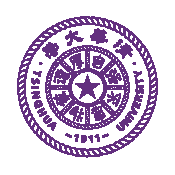
\includegraphics[height=3cm]{thu-fig-logo}}%
  \hspace{4em}%
  \subcaptionbox{第二个小图形,注意这个图略矮些。如果标题很长的话,它会自动换行\label{fig:subfig2}}
      {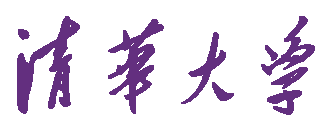
\includegraphics[height=2cm]{thu-text-logo}}
  \caption{包含子图形的大图形(subcaptionbox示例)}
  \label{fig:big1-subcaptionbox}
\end{figure}
\begin{figure}[h]
  \centering%
  \begin{subfigure}{3cm}
    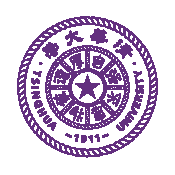
\includegraphics[height=3cm]{thu-fig-logo}
    \caption{第一个小图形}
  \end{subfigure}%
  \hspace{4em}%
  \begin{subfigure}{0.5\textwidth}
    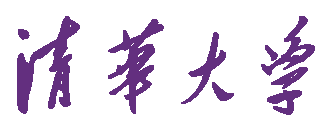
\includegraphics[height=2cm]{thu-text-logo}
    \caption{第二个小图形,注意这个图略矮些。subfigure中同一行的子图在顶端对齐。}
  \end{subfigure}
  \caption{包含子图形的大图形(subfigure示例)}
  \label{fig:big1-subfigure}
\end{figure}

古之学者必有师。师者,所以传道受业解惑也。人非生而知之者,孰能无惑?惑而不从师,
其为惑也,终不解矣。生乎吾前,其闻道也固先乎吾,吾从而师之;生乎吾後,其闻道也亦
先乎吾,吾从而师之。吾师道也,夫庸知其年之先後生於吾乎!是故无贵无贱无长无少,道
之所存,师之所存也。

嗟乎!师道之不传也久矣,欲人之无惑也难矣。古之圣人,其出人也远矣,犹且从师而问焉;
今之众人,其下圣人也亦远矣,而耻学於师。是故圣益圣,愚益愚。圣人之所以为圣,愚
人之所以为愚,其皆出於此乎?爱其子,择师而教之,於其身也,则耻师焉,惑焉。彼童子
之师,授之书而习其句读者,非吾所谓传其道、解其惑者也。句读之不知,惑之不解,或师
焉,或不焉,小学而大遗,吾未见其明也。巫医、乐师、百工之人不耻相师,  士大夫之族
曰“师”曰“弟子”之云者,则群聚而笑之。问之,则曰:彼与彼年相若也,道相似也,位
卑则足羞,官盛则近谀。呜呼!师道之不复,可知矣。巫医、乐师、百工之人。吾子不齿,
今其智乃反不能及,其可怪也欤!圣人无常师。孔子师郯子、苌子、师襄、老聃。郯子之徒,
其贤不及孔子。孔子曰:“三人行,必有我师。”是故弟子不必不如师,师不必贤於弟子。
闻道有先後,术业有专攻,如是而已。

如果要把编号的两个图形并排,那么小页就非常有用了:
\begin{figure}
\begin{minipage}{0.48\textwidth}
  \centering
  
\includegraphics[height=2cm]{thu-whole-logo}
  \caption{并排第一个图}
  \label{fig:parallel1}
\end{minipage}\hfill
\begin{minipage}{0.48\textwidth}
  \centering
  
\includegraphics[height=2cm]{thu-whole-logo}
  \caption{并排第二个图}
  \label{fig:parallel2}
\end{minipage}
\end{figure}

李氏子蟠,年十七,好古文、六艺,经传皆通习之,不拘於时,学於余。余嘉其能行古
道,作师说以贻之。

\hfill —— 韩愈(唐)



%%% 其它部分
\backmatter

%% 本科生要这几个索引,研究生不要。选择性留下。
% 插图索引
\listoffigures
% 表格索引
\listoftables
% 公式索引
\listofequations


%% 参考文献
% 注意:至少需要引用一篇参考文献,否则下面两行可能引起编译错误。
% 如果不需要参考文献,请将下面两行删除或注释掉。
\bibliographystyle{thuthesis}
\bibliography{ref/refs}


%% 致谢
% 如果使用声明扫描页,将可选参数指定为扫描后的 PDF 文件名,例如:
% \begin{ack}[scan-statement.pdf]
\begin{acknowledgement}
  衷心感谢导师 李洪波 老师对本人的精心指导。他不仅是我的毕设指导老师,还是我的班主任和任课老师,在我的整个大学期间对我的学业,学术,乃至日常生活都起了极大的帮助作用,他平易近人的作风,关心学生的热情以及对待工作的忱将使我终生受益。

  感谢清华大学智能技术与系统国家重点实验室,以及实验室全体老师和同学们在我毕设工作中的热情帮助和支持。

  感谢清华大学计25班的各位大神,你们的存在使我的本科轻松快乐了许多。

  感谢 \thuthesis,它让我可以专心于论文的内容而非格式,使我的毕设论文工作轻松了许多。
\end{acknowledgement}


%% 附录
\begin{appendix}
% \newgeometry{left=2cm}
\chapter{外文资料原文}
\label{cha:engorg}

\title{Multimodal Deep Learning for Robust RGB-D Object Recognition}
\begin{center}
{\footnotesize Andreas Eitel, Jost Tobias Springenberg, Luciano Spinello, Martin Riedmiller, Wolfram Burgard}
\end{center}

\begin{figure}[ht]
   \centering
     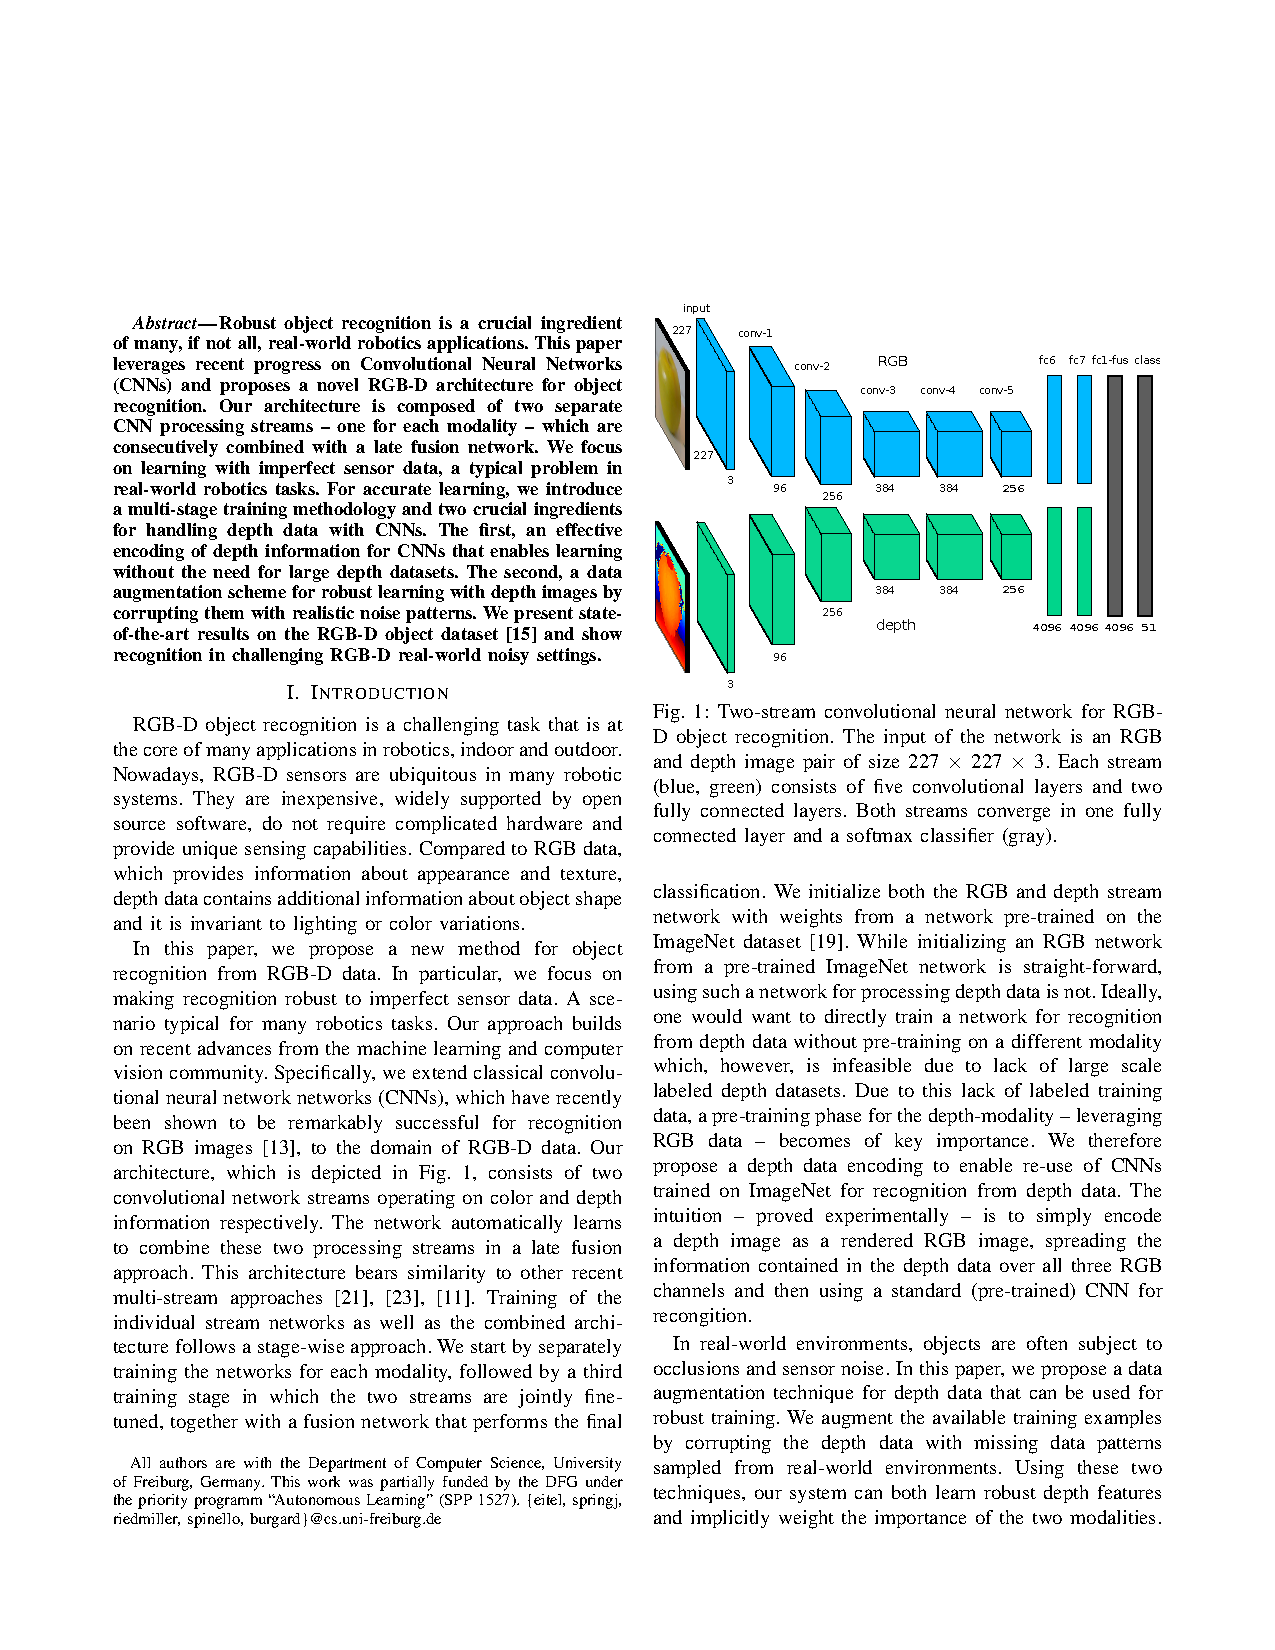
\includegraphics[page=1,width=0.95\textwidth]{MultimodalRGBD}
\end{figure}

% \restoregeometry

\begin{figure}[ht]
   \centering
     \includegraphics[page=2,width=0.95\textwidth]{MultimodalRGBD}
\end{figure}

\begin{figure}[ht]
   \centering
     \includegraphics[page=3,width=0.95\textwidth]{MultimodalRGBD}
\end{figure}

\begin{figure}[ht]
   \centering
     \includegraphics[page=4,width=0.95\textwidth]{MultimodalRGBD}
\end{figure}

\begin{figure}[ht]
   \centering
     \includegraphics[page=5,width=0.95\textwidth]{MultimodalRGBD}
\end{figure}

\begin{figure}[ht]
   \centering
     \includegraphics[page=6,width=0.95\textwidth]{MultimodalRGBD}
\end{figure}

\begin{figure}[ht]
   \centering
     \includegraphics[page=7,width=0.95\textwidth]{MultimodalRGBD}
\end{figure}

\chapter{外文资料的调研阅读报告或书面翻译}

\title{\heiti 多模态深度学习与稳定的RGB-D物体识别}

{\heiti 摘要:}
稳定的物体识别是许多现实世界中机器人应用问题中的关键因素。本文基于卷积神经网络(CNN)的最新进展,提出了一种新型的RGB-D物体识别架构。我们的体系结构是由两个独立的CNN处理流组成的——每个模态对应一个处理流——并继续与后期的融合网络相结合。我们关注不完美的但是在现实世界经常遇到的有噪音的传感器数据。为了获得准确的学习,我们引入了一个分级的训练方法和两个适用于CNN的用来处理深度数据的技巧。第一个技巧是,使用一种对CNN有效的深度信息编码,使学习不需要很大的深度数据集。第二个技巧是,使用一种适用于深度信息的数据增强方法,用现实的噪音模式破坏它们。我们提出的识别架构在RGB-D物体数据集[15]上获得了最先进的识别成果,并且在富有挑战性的现实世界RGB-D数据中也获得了较好的识别结果。

\section{引言}

RGB-D物体识别是一项具有挑战性的任务。它在机器人领域以及室内和室外的许多应用中都是核心技术。如今,RGB-D传感器无处不在。许多机器人系统都可以使用价格便宜,广受支持的开源软件,而不需要使用复杂的硬件来提供独特的感知能力。RGB数据,提供了有关外观和纹理的信息;而深度数据则包含有关物体形状的附加信息,它是不随亮度或颜色而改变的,所以对物体识别具有特殊的意义。

在本文中,我们提出了使用RGB-D数据的新的对象识别方法。特别是,我们关注在有噪声的情况下——一个典型的机器人任务的背景下——稳健地识别不完善的传感器数据。我们的方法建立在机器学习和计算机视觉的最新研究成果上。具体地说,我们扩展了经典的卷积神经网络(CNN),CNN最近被证明在RGB图像[13],以及RGB-D数据识别方面获得了显着的成功。我们的工作的结构如图 1所示。由两个关于颜色和深度操作卷积网络流分别处理两种信息。由网络自动学习这两种处理流在后期的融合策略。这种架构与其他最近的多流的方法[21],[23],[11]相比有着比较大的相似度。将训练出来的单个网络流以及将合并的部分使用分阶段训练的方式是很有效果的。我们启动训练网络分别对于每个模态,以及两个模态融合的阶段训练微调,与执行网络连接,最终的融合网络会做出最总的分类结果预测。我们初始化RGB和深度流网络所用的权值是从一个在ImageNet数据集[19]上预先训练好的神经网络模型继承来的。尽管我们可以直接使用这个在颜色信息中训练好的模型来分类RGB信息,但是并不能直接使用它来分类深度信息。理想情况下,我们可以直接使用深度数据训练出一个适合的CNN模型,而不用使用其它模态的数据。然而,实际中是不可行的,因为缺乏大量已经标记的深度数据集。由于缺乏标记的训练的数据,深度模态在训练的初始状态需要借鉴使用RGB数据训练出的模型,这是至关重要的。因此,我们提出了一种深度数据编码,以便再利用在ImageNet中训练好的CNN来识别深度数据。这个已经被试验验证的直觉是简单地将深度图像编码作为RGB图像,在三个RGB信道中都填上深度数据的信息,然后使用标准(预训练的)CNN做识别。

在现实环境中,对象是经常受到遮挡和传感器噪声的影响。在本文中,我们提出了一种深度数据增强技术,该技术可用于有噪声场景的稳定的训练。我们增加了训练样例,通过使用从现实环境采样的缺失数据型态来破坏深度数据。使用这两种技术,我们的系统既可以学习稳定的的深度识别和隐式加权两种模式的重要性。
 
我们测试了我们的方法来验证我的想法:我们在RGB-D的数据集中使用我们的方法做分类以测试我们方法的精度,然后在有现实世界噪音的数据集中测试我们方法的稳健性。对于第一个,我们的实验结果表明,我们的工作性能优于所有现有技术在Lai等人的RGB-D对象数据集[15]中的分类结果。第二,我们表明我们的数据增强方法提高了在充满挑战的现实世界和有噪声条件下的RGB-D场景的数据集[16]中的识别准确率。

\section{相关工作}

我们的做事涉及到两块重要的工作,分别是卷积神经网络(CNN)用来做物体识别,和应用计算机视觉的方法去解决使用RGB-D数据做识别中遇到的问题。尽管本文不会做一个包含CNN和物体识别的综合广泛的文献综述,我们还是会快速的点明我们的方法和近期已有的工作有什么区别。

在众多成功的RGB-D物体识别算法中,有很大一部分都是使用手工设计的信息,比如SIFT与深度信道的多种形状特征结合 [15],[16]。然而,随着它们在许多计算机视觉的问题中都获得了成功,非监督学习的特征学习方法也在最近被拓展到了RGB-D识别的领域。Blum等人[3]提出了一种基于K-Means的RGB-D描述符。更加近期的工作包括Bo等人[5]提出的分层匹配追踪,一种分层级的稀疏编码方法,可以从多个输入信道学习特征。Socher等人[22]提出了一种不同的方法,这种方法依靠将卷积过滤器和递归神经网络(一种特殊的再现神经网络)结合起来作为识别层级。Asif等人[1]报告了一种可以使用随机森林瀑布来提高识别准确率的分类器,这种分类器也是分层融合的。最后,在最近Schwarz等人的独立工作中[20],提出了使用ImageNet上预先训练出的CNN提取出的RGB-D特征来做RGB-D识别。尽管他们也使用有两个网络流组成的分类架构,他们并没有对CNN使用RGB-D做微调,而只是使用原有的神经网络。有趣的是,他们还发现了简单的上色方法可以使深度信息获得较好的识别效果,甚至可以与许多复杂的预处理的效果相当。与他们的工作不同,我们获得了更高的准确率,并且训练出一个端对端的融合CNN:输入未加工的像素信息,直接输出分类信息,整个过程是一个监督学习的过程,并且使用了在相关任务中训练的模型。所以,我们的CNN学习到的特征从结构上与现有的其他任务中的特征是可区分的。使用CNN做物体识别在计算机视觉和机器学习领域有着很长的历史。尽管人们都知道CNN在监督的图像识别、分类任务中(比如MNIST [17])很早就可以获得较高的准确率,最近CNN方法已经不仅仅可以在例如大规模图例如分类任务[13]、物体识别[9]、语义分割[8]等方面中超过经典的方法,还可以产生在多种任务中转换的特征[7],[2]。计算能力强大的高性能计算系统使得这个最近的成功的故事成为可能,而大规模图像数据集的出现也起了不可或缺的作用,比如ImageNet[19]。




虽然大多数的深度学习工作的重点是二维图像,最近的研究也已经包含使用深度信息用于改进场景分类和物体检测[6],[10]。其中,和我们最相似的是Gupta等人[10]提出的比较普适的使用R-CNN检测器适用于深度信息的方法[9]。详细地说,他们使用已经在RGB图片数据集上训练好的大型CNN去提取深度信息中的特征,将深度信息编码到三个信道(使用HHA编码)。更加具体地说,他们对每一个像素点,编码了离地面的高度,水平的距离和像素层面上的表面法向和重力之间的角度。我们的融合网络架构与他们的使用预先训练的神经网络有着相似之处。不过我们的方法与他们的方法的不同之处在于,将深度信息编码为颜色信息的过程和融合两种模态的融合方法。对于编码过程,我们提出了一种对于深度图片的编码方法,我们的这种方法不依赖于复杂的预处理,但是与HHA相比获得了性能上的改进。为了实现模态融合,我们在原有神经网络的基础上有加了一层融合层,使得我们的识别架构可以自动的学习出对于识别的融合的策略,这和仅仅在提取出的信息的上面训练出一个线性分类器先比有着更好的表现。多刘的架构已经被人用于多种任务,包括识别[21],检测[11],图片提取[23]。一个最近的有关深度和图片信息融合的不同网络结构在Saxena等人的研究中给出[18]。在哪里,作者比较了不同的多模态学习的模型:
\begin{enumerate}
\item 早期融合,其中输入图像被级联到现有的图像RGB通道并一起处理;
\item 我们定义为后期的融合,其中的功能是为每个单独训练的情态,然后在更高层融合;
\item 将早期和晚期的方法结合;
\end{enumerate}
得出的结论是后期融合(2)和早期和后期相结合的办法最适合把握问题的关键特征,有利于检测。相比与他们的工作,我们的模型是使用类似于后期融合的方法,但又有着很大的不同。[18]使用逐层无人监督的训练方法,他们的规模(包括其网络和输入图像数据集的大小
)都比我们要小一个数量级。

\section{用于RGB-D物体识别的多模态架构}

该架构的概述在图 1中给出。 我们的网络由两个流(在图 1中的顶部蓝色和底部绿色)——分别处理RGB和深度数据——然后在更晚的阶段被融合在一起的方法。每个流由一个已经在ImageNet数据集中训练好的深度CNN组成(我们使用Krizhevsky等人[13]训练的CaffeNet[12]作为预训练模型)。使用预先训练的神经网络的关键原因是我们希望在优先的数据量上使用一个包含着百万级别的参数的大型CNN。(例如,见Yosinski等人 [25]在最近对于此的讨论)我们首先对两个模态的信息进行预处理,然后使用分阶段的方法训练我们的多模态CNN网络。我们首先对每个模态的CNN进行微调,然后使用两个模态微调出的模型,将它们结合在一起,联合的训练出融合网络的参数。不同的步骤将会在一下小节被详细说明。

\subsection{输入预处理}

要充分利用在ImageNet上预先训练的CNN的力量,我们预处理RGB和深度模态的输入数据,使得它与原ImageNet的输入兼容。具体地说,我们使用在CaffeNet[12]中的参考实现,这个模型接受227 $\times$ 227像素的RGB作为输出。这227 $\times$ 227个像素点通常是用256 $\times$ 256个像素点的RGB图片缩放而成的。处理的第一步要缩放图片到合适的大小。而缩放最简单的方法就是使用图片翘曲,放弃原始图片的长宽比例直接缩放。这在图片3(中)中有所阐释。我们发现在我们的试验中,这个处理过程会降低识别的准确率——我们把这个问题归因于目标物体形状信息的损失(见IV-C)。所以我们设计了一种不同的预处理方法:将长边缩放到256个像素,得到一个256 $\times$ N或者 N $\times$ 256的图片。然后我们将缩放后的图片沿短边像瓷片一样平铺到256 $\times$ 256的空间上。得到的最终的颜色图片和深度图片在物体边界处展示出一种人造的环境(见图 3)。我们对颜色信息和深度信息都是用这种方法进行预处理。

对于RGB图像,在预处理缩放之后可直接使用作为CNN的输入,而缩放之后的深度数据需要额外的步骤。为了实现这一点,我们可以回想一下是用ImageNet训练的神经网络已经被训练去识别某个特别的图像输入分布(即天然相机图像),它与深度传感器得到的标志物体距传感器的距离的信息是不相容的。尽管如此,通过查看一个典型的家用物品的深度图片(参考图 4),可以得出结论,许多定性
出现在RGB图像中的特征,比如边、角、阴影区域等模式,也会出现在深度图片中。这种认识引出了这种想法:简单地使用深度数据渲染出的三通道的RGB图片作为用于在ImageNet [10]上训练的CNN的输入。我们将比较这些深度图片渲染的方法与我们的做法的不同之处。两种最流行的深度图片编码是:
\begin{enumerate}
\item 深度数据渲染成灰度值,并复制灰度值到所要求的三个通道作为神经网络输入;
\item 利用表面法线,其中每个法线矢量的维度对应于一个信道所产生的图像。
\item 一个更复杂的方法,称为HHA编码[10],对每一个像素点的三个信道,编码了离地面的高度,水平的距离和像素层面上的表面法向和重力之间的角度。
\end{enumerate}


我们提出第四种有效并且计算成本较低的,将信息编码为彩色图像的方法,我们发现此种方法在物体识别中的表现要比HHA编码更好。我们的方法首先要标准化所有的深度值到0和255。然后,我们应用一个喷射颜色表将深度信息从单通道输入转换到一个三通道图像(给深度着色)。对于尺寸为 W $\times$ D 的深度图像中的每个像素(i,j)中,我们将距离信息映射为颜色值,从红色(附近)到绿色再到蓝色(远),并将这些信息分散到三个信道。这三个信道的边缘往往对应着有用的对象边界。因为我们使用的卷积神经网络是用RGB图像训练的,着色过程提供了深度信息和RGB图像之间足够多的共同结构,所以可以使用CNN来处理深度信息(对不同深度预处理方法之间的比较参照图 2)。

\section{实验}

我们在华盛顿大学的RGB-D物体数据集[15]上评估对我们的多模态神经网络体系结构。这个数据集包括属于51个不同类别的日常家用物品。作为额外实验,我们使用了RGB-D场景数据集中的被部分遮挡的物体来评估的算法的可靠性以及对于现实世界数据的分类能力。

\subsection{实验设置}

所有实验都是使用开源的Caffe框架[12]。如先前所描述,我们使用
的CaffeNet作为我们融合网络的基础。它由五个卷积层(在第一、第二和第五之后需要最大池化),其次是两个完全连接层和SOFTMAX分类层。除了最后一层之外所有的层都用到了修正线性单元。我们使用预先训练的模型的前八层的权重和偏差来初始化我们网络的前八层,丢掉了最后的SOFTMAX分类层。然后我们继续使用分阶段训练。第一阶段(分别训练RGB和深度信息)当中所有信息层的参数都按照一种固定学习率(learning rate)的模式在改变(最开始学习率取为0.01,经过20K次迭代后变为0.001,并在30K次迭代后停止训练)。在第二阶段(训练融合网络,20K次迭代,使用大小为50的mini-batch),我们尝试微调了所有的权值,但是最后发现将上一阶段训练出的两个模态的各自的CNN网络权值固定(设定它们的学习率为0),只微调融合部分的网络效果更好。我们从此任务的十种数据分割方法中随机选出一种分割作为确认分割,而训练的迭代次数是基于在确认分割上的测试结果所选定的。如果没有特殊说明,我们使用固定为0.9的momentum和固定为128的mini-batch。我们还使用了常见的数据增强的做法:在较大的256 $\times$ 256的图片中随机选取大小为227 $\times$ 227子图像,然后实行随机水平翻转。我们使用一块NVIDIA 780显卡,训练单支神经网络流需要10个小时。

\subsection{RGB-D物体数据集}

华盛顿RGB-D数据集的物体由41877个含家用物品RGB-D图像组织成,它们分别属于51个不同的种类的一共300个实例。这些图像是在三个不同视点捕捉的。我们使用间隔5帧的采样来评估我们的算法。我们使用和Lai等
人 [15]相同的十折交叉验证分割,来评估我们的方法在具有挑战性的类别识别任务中的表现。每个分割包括大约35000组训练图像和7000组测试图像。每一个对象类中,一个是被留下做测试的。所以我们在剩下的300-51 = 249个实例中进行训练。在测试时CNN的任务是给每个之前没见过的实例分类。

表I显示了我们的多模态CNN识别的平均准确率与以往工作中的最好结果的对比。
我们得到的最佳结果,使用喷射着色(FUS-CNN JET)与RGB和深度信息时(84.1 $\pm$ 2.7\%和83.8 $\pm$ 2.7\%时,当分别使用RGB或深度模式时),得到的91.3 $\pm$ 1.4\%的整体准确率,比就我们所知的所有前人的工作都要高。
我们还展示了使用需要更多计算的HHA编码的结果(FUS-CNN HHA)。从表中可以看出,HHA编码并没有带来表现的提升。我们提出的着色方案要比HHA的表现(FUS-CNN HHA)稍好一点,同时需要更少的计算资源。整体来说我们的试验结果表明,一个预先训练的CNN可以用来识别深度数据,只需要预先使用我们的着色方法对深度信息进行预处理即可。除了表中展示的结果,我们还做了有关不不同的融合网络结构的试验。具体来说,如果将融合中间层(fc1-fus)去掉,识别准确率会稍微下降至91\%。增加融合层也不能得到更好的结果。最终,图6展示了每个类的召回率(recall),其中大约一半物体实现了约等于99\%的召回率。

\subsection{深度域适应RGB-D场景}

为了测试我们的深度信息增强方法在真实世界中的效果,我们进行了在更具挑战性的RGB-D场景数据集中的附加实验。此数据集包括六个对象类(与RGB-D物体数据集重叠)和大量受噪声影响的深度图像。在这个实验中,我们训练的两个单流深度神经网络,使用物体数据训练,并使用场景数据集进行测试。
此外,我们假设一定正确的边框已经被给出,这种就可以只测试识别的性能。第一个“基准”神经网络由第III-B.1中描述的方法所训练出来,标签的总数目M = 6。第二神经网络是使用III-C中提出的深度信息增强方法训练出来。
该实验的结果展示于表II(中间和右栏),报告了每个对象类在所有八个视频序列中的识别精度。
从该表中可以看出,经过适应的网络是明显的(右边使用数据增强方法训练的列)优于基准模型中的所有类,这显然表明额外的领域适应性对于在现实世界中的场景的稳健识别是有必要的。
然而,一些类(例如,盖,碗,苏打罐)从噪音训练中获得提升比其他类更高(例如,手电筒和咖啡杯)。图 4中描绘的厨房场景给出了一些有关此结果的视觉直觉。
另一方面,一些对象(例如,汽水罐)往往会出现非常嘈杂对象边界和表面,因此它们使用适应方法会显示出较大的识别性能改进。
另一方面,小物体(例如,手电筒),这些物体经常是在桌子上拍的,要么不受噪音影响或只受轻微的影响,因此这些噪音容易被我们的数据增强方法完全擦除。图 7显示了几个被基准网络错误分类,但是可以使用我们的数据增强方法正确分类的例子。
我们还测试了如图 3所描述的不同的图像缩放技术的效果。如表II所示,标准图像变形表现的不是很好,这支持了我们的直觉,即形状信息会在预处理过程中丢失。

\subsection{深度编码方法的比较}

最后,我们进行了实验,以比较图 2所描述的不同的深度编码及方法。对于图像的缩放,我们使用了图 3描述的需处理方法,并使用不同的深度信息编码方法进行了测试。
我们考虑到两种场景:
\begin{enumerate}
\item 使用单通道深度图像做训练
\item 对每一种编码方法,只使用第三节-B.1的方法来预处理深度信息,然后作为训练集。
\end{enumerate}
当从头训练时,初始学习率设定为0.01,然后在40K次迭代后改变到0.001。经过反复迭代60K次后停止。训练更多的迭代次数并不能进一步提高精度。通过查看表III中的结果,很显然训练从头训练的表现不如使用已有模型微调的效果好。在后一种情景下,结果显示最简单的编码方式(将深度信息转换为灰度图片)的识别效果要显著差于其他的方法。在其他的编码方法中(所有这些方法都会给深度信息着色),平面法向和HHA编码需要额外的图片图像预处理,而使用我们提出的深度-喷射着色的方法几乎不需要任何计算资源。一个HHA编码在此情景下表现的不尽人意的可能原因是此数据库中的图片都是放在一个可以旋转的托盘中,他们的高度都是相同的。所以HHA中用到的高度信道就无法包含用于分类的其他信息。在本实验中,使用平面法线要比深度-jet编码的表现稍好一点。所以我们使用平面法线的编码来试验了我们的融合网络,不过这并没有进一步提高识别表现。具体地说,测试集上的识别准确率是91.1 $\times$ 1.6,这与我们在表I中报告的结果相差不大。

\section{结论}

我们提出了一种可以用于RGB-D物体识别,并且在RGB-D物体数据集[15]中实现了当前最好表现的新型多模态神经网络结构。我们的方法是由二个卷积神经网络流组成,这两个CNN流在分类前可以从RGB和深度信息中自动地提取和融合信息。我们利用一种有效的编码方式,把深度数据编码为图像,使我们能够充分利用在ImageNet数据集中训练的大型神经网络进行对象识别。我们提出了一种新的深度数据增强方法,旨在提高对嘈杂的现实世界深度数据的识别准确率,以便适用于典型的机器人场景。目前大量的实验结果证明了我们方法的正确性,以及它能够从两个模态学习丰富的特征。我们的方法还可以在现实世界环境中稳定地识别物体,并证明了噪声感知训练是有效的,并且可以被用来改进RGB-D场景数据集[16]的识别精度。
\end{appendix}

%% 个人简历
\begin{resume}

  \resumeitem{个人简历}

  1993 年 06 月 10 日出生于 黑龙江 省 大庆 市。

  2012 年 9 月考入 清华 大学 计算机科学与技术 系攻读 计算机科学与技术工学学士 学位至今。

  \researchitem{发表的学术论文} % 发表的和录用的合在一起

  % 1. 已经刊载的学术论文(本人是第一作者,或者导师为第一作者本人是第二作者)
  \begin{publications}
    \item \textbf{Gao B}, Li H, Li W, et al. 3D Moth-inspired chemical plume tracking and adaptive step control strategy[J]. Adaptive Behavior, 2016: 1059712315623998.
    \item \textbf{Gao B}, Li H, Sun F. 3D moth-inspired chemical plume tracking[C]//2015 IEEE International Conference on Robotics and Biomimetics (ROBIO). IEEE, 2015: 1786-1791.
  \end{publications}

\end{resume}

\end{document}
